\section{Spinning ellipse}
\label{section:Spinning_ellipse}
\subsection{Drag and lift}
For the spinning elliptic bodies, we look at nondimensional drag and lift force, rather than drag and lift coefficients. This is because the frontal area needed to calculate coefficients varies with time. For simplicity and consistency, we look at nondimensional forces rather than coefficients. We begin looking at the results of the spinning ellipses by observing the cycle average plots of drag and lift to see the general trends. We briefly neglect the noise from shape-phase effects to help us identify under which parameters vortex-shedding occurs. Fig. \ref{fig:mvmean1p5} and \ref{fig:mvmean0p5} show the cycle-averaged drag and lift for the two ellipse cases. These plots show oscillation about the mean. We take the cycle-averaged values and divided by their respective averages and subtracted one. This way we can see the oscillation about the mean. We observe that even when we transform the shape of the body to a noncircular shape, we still find similar relations between flow regime and $Fr^2$. We find other similarities to the circle cases. We witness when $Fr^2 > 0.1$, there is no steady-state value. A transition occurs around $t = 100$ in the $Fr^2 = 10$ cases. The drag and lift undergo a small but distinct decrease. At $Fr^2 = 1$ there is an unsteady transition regime. 

Moving on from comparison with the circle cases, we observe vortex-shedding occurs at $Fr^2 > 1$. At $Fr^2 = 10$, it takes longer for the drag and lift values to reach a quasi-steady-state flow regime. Now that we have looked at the general trends in drag and lift, we move to looking at phase-averaged results. Figures \ref{fig:pa1p5} and \ref{fig:pa0p5} show the phase-averaged drag results for the elliptic shapes. 

An interesting insight is how at $Fr^2 = 0.1, 0.01$, in the cycle average plots, there is no oscillation , but in the phase average plots, these $Fr^2$ numbers have the largest amplitudes of oscillation. At high stratification, the vortex-shedding is suppressed, but through spinning the body overcomes large potential energy barriers to rotate. The resistance from the potential energy barrier manifests in the large amplitudes of phase-oscillation in drag and lift. Just like the ensemble average plots show, the effect of stratification on mean drag at $Fr^2 < 1$ is substantial. These effects are quantified in tables \ref{tab:fd} and \ref{tab:fl}, which show the mean, minimum, and maximum drag and lift values for the ellipses. An interesting phenomenon is how a decrease in stratification not only reduces drag, but causes it to go negative to produce thrust.  This phenomenon of thrust was previously observed in unstratified flow simulations in literature \cite{lua_rotating_2018}. Increase in stratification causes a decrease in lift. Whereas when the stratification was higher, the only substantial low-pressure zone for the ellipses was on the top, with high stratification there are low pressure zones on the top, bottom, and to the right. This explains the decrease in lift with increase in stratification for the ellipses. This is shown in figures \ref{fig:ar1p5_pressure} and \ref{fig:ar0p5_pressure}.

Another effect of increasing stratification that is found in the phase-averaging plots is the change in phase. At $Fr^2 < 1$, there is a phase-lag that increases as stratification increases. This phase-lag is larger with lift than with drag. Tables \ref{tab:max_drag} and \ref{tab:max_lift} show the angles of maximum drag and lift and help us quantify this phase-lag. The phase differences in drag from $Fr^2 = \infty$ to $Fr^2 = 0.01$ are slightly higher for lift than for drag. They are also slightly higher for the case of $AR = 1.5$ than for $AR = 0.5$. 
 
\begin{figure}
    \centerline{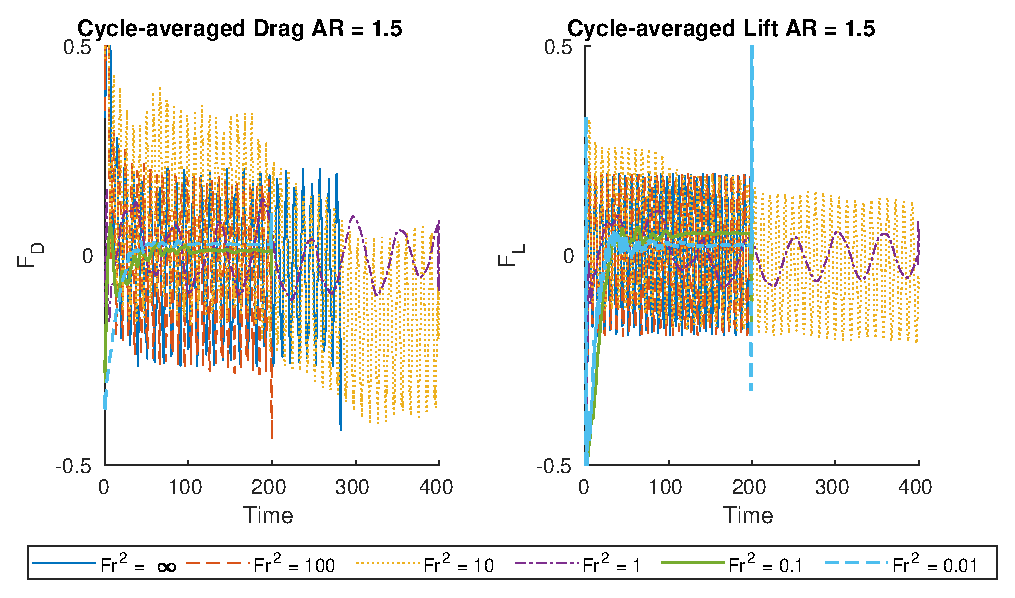
\includegraphics[width=\textwidth]{images/spinning_ellipse/mvmean1p5.eps}}
    \caption{Drag and lift over time averaged across each period for $AR = 1.5$}
    \label{fig:mvmean1p5}
\end{figure}

\begin{figure}
    \centerline{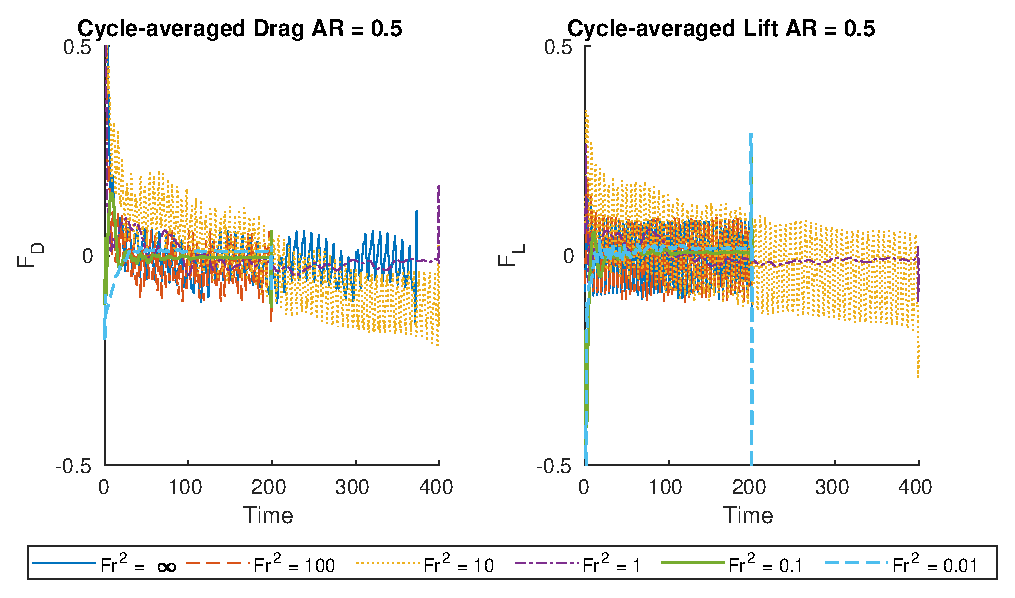
\includegraphics[width=\textwidth]{images/spinning_ellipse/mvmean0p5.eps}}
    \caption{Drag and lift over time averaged across each period for $AR = 0.5$}
    \label{fig:mvmean0p5}
\end{figure}

\begin{figure}
    \centering
    \begin{subfigure}[b]{0.49\textwidth}
        \centering
        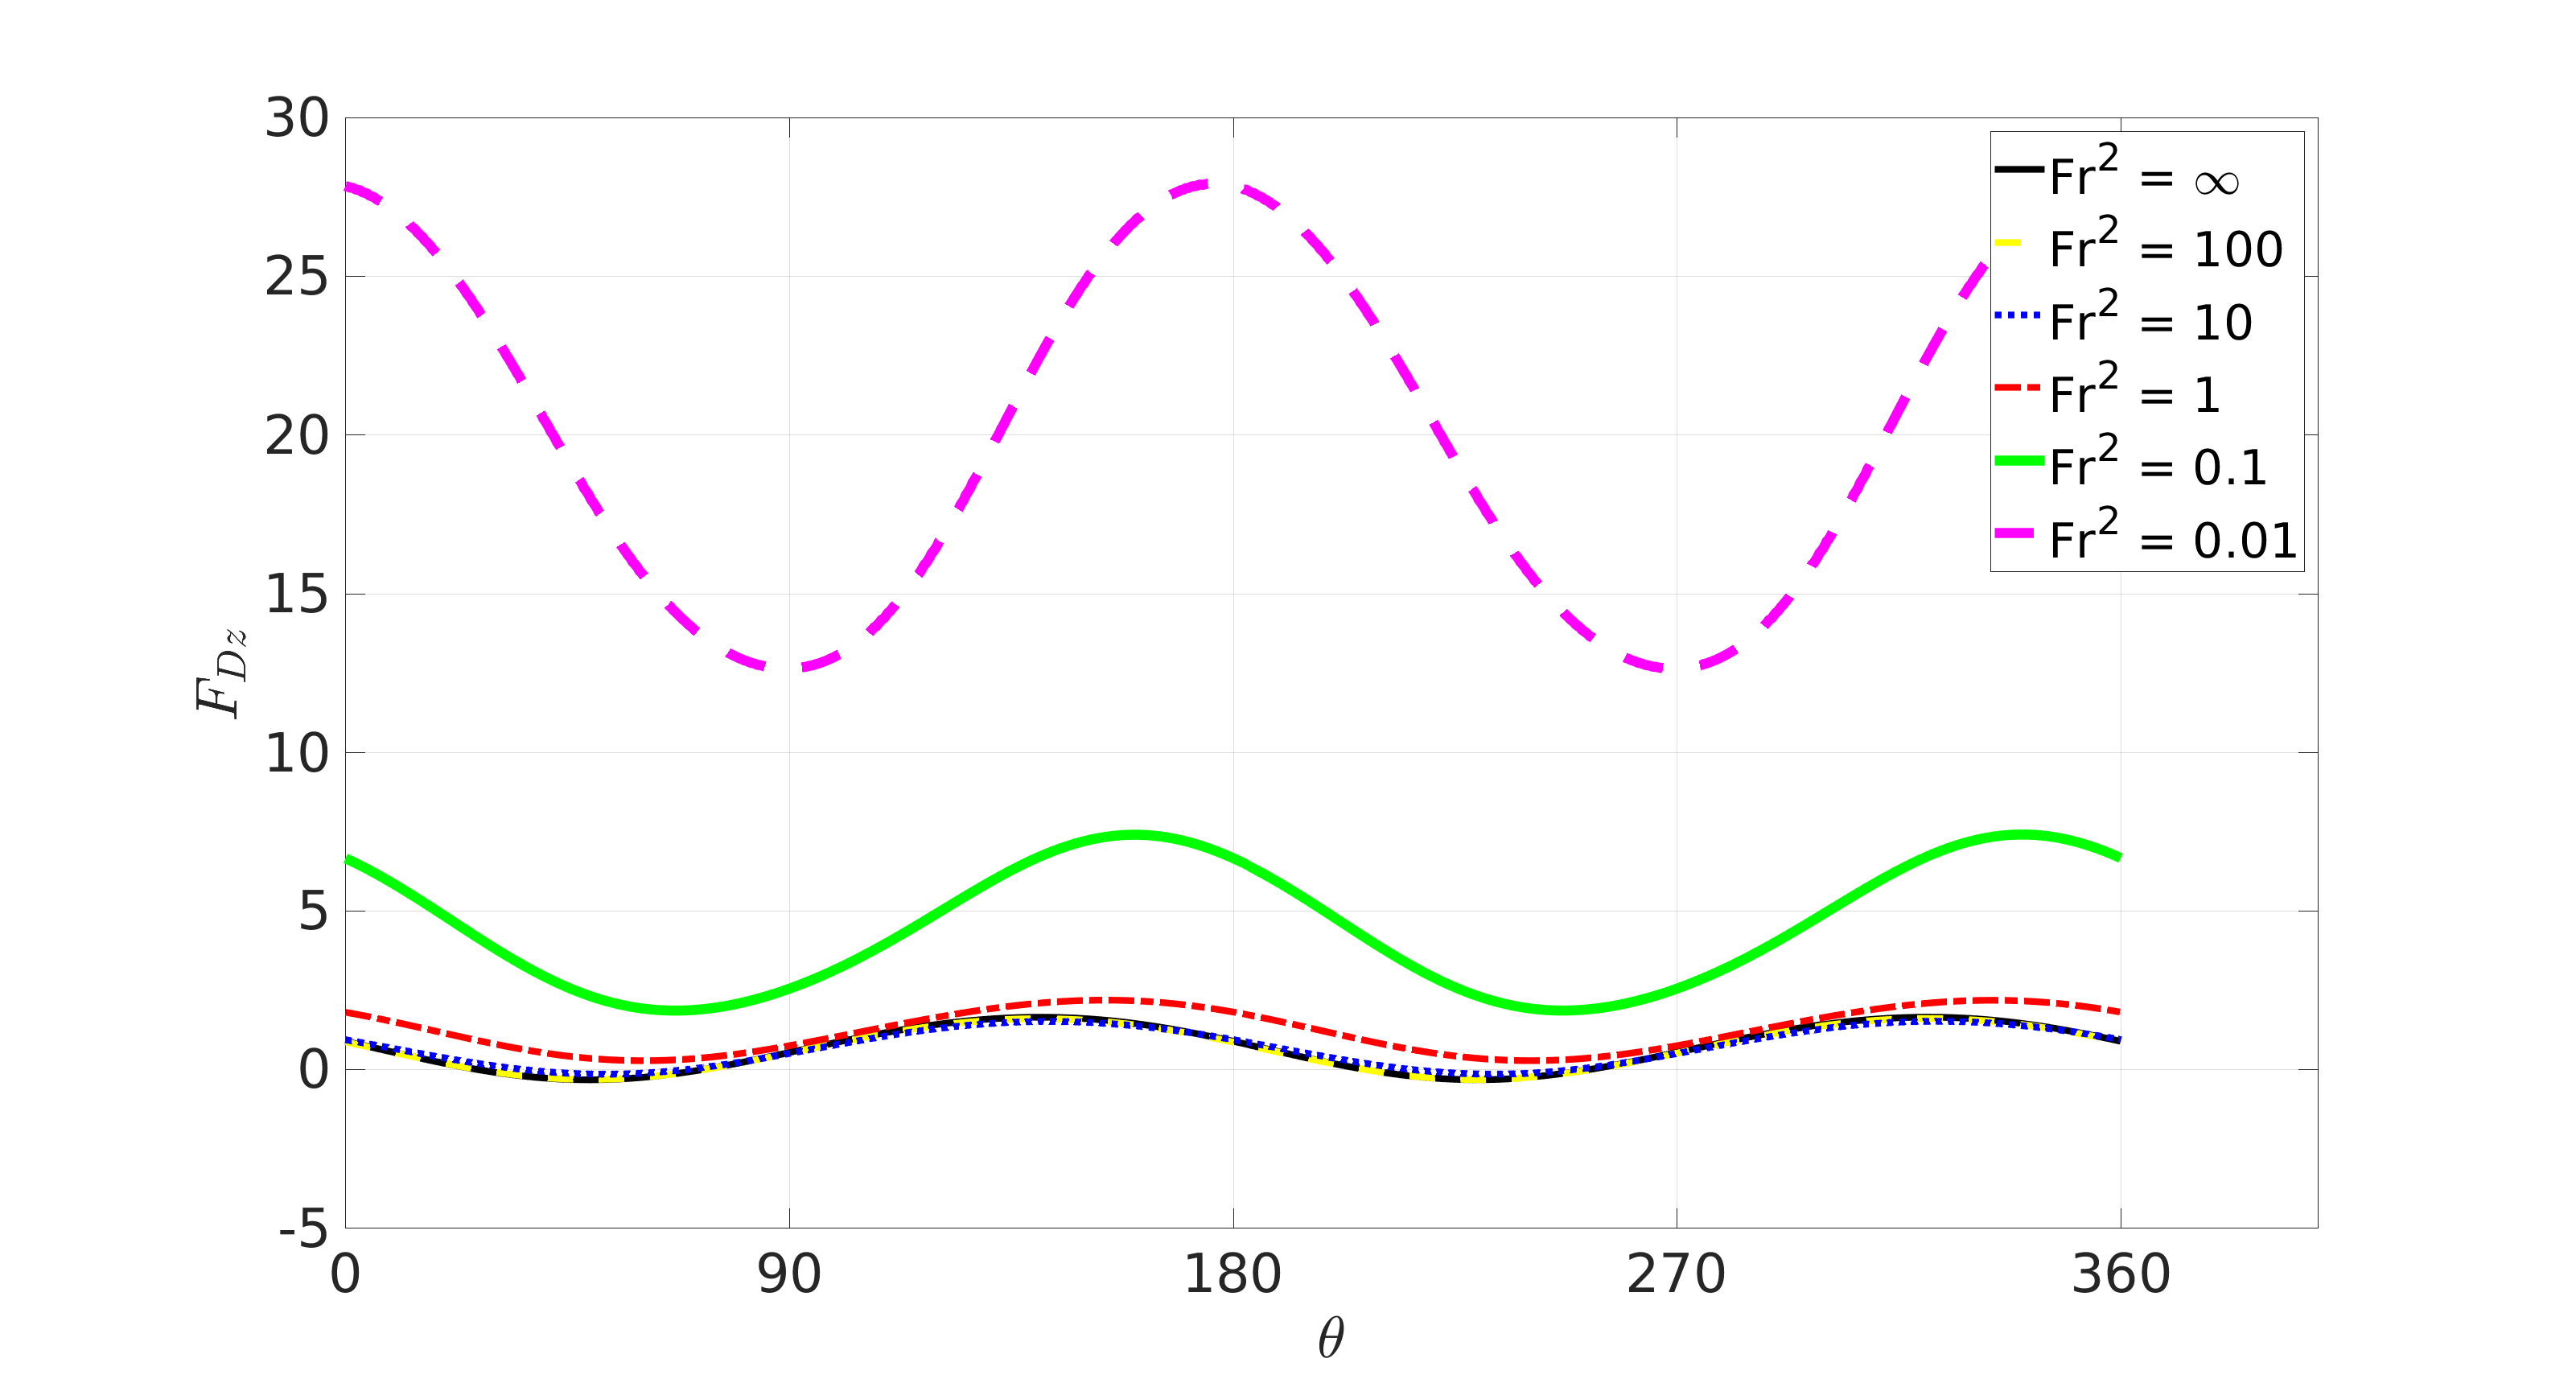
\includegraphics[width=\textwidth]{images/spinning_ellipse/padrag1p5.eps}
        \caption{}
        \label{fig:padrag1p5}
    \end{subfigure}
    \hfill
    \begin{subfigure}[b]{0.49\textwidth}
        \centering
        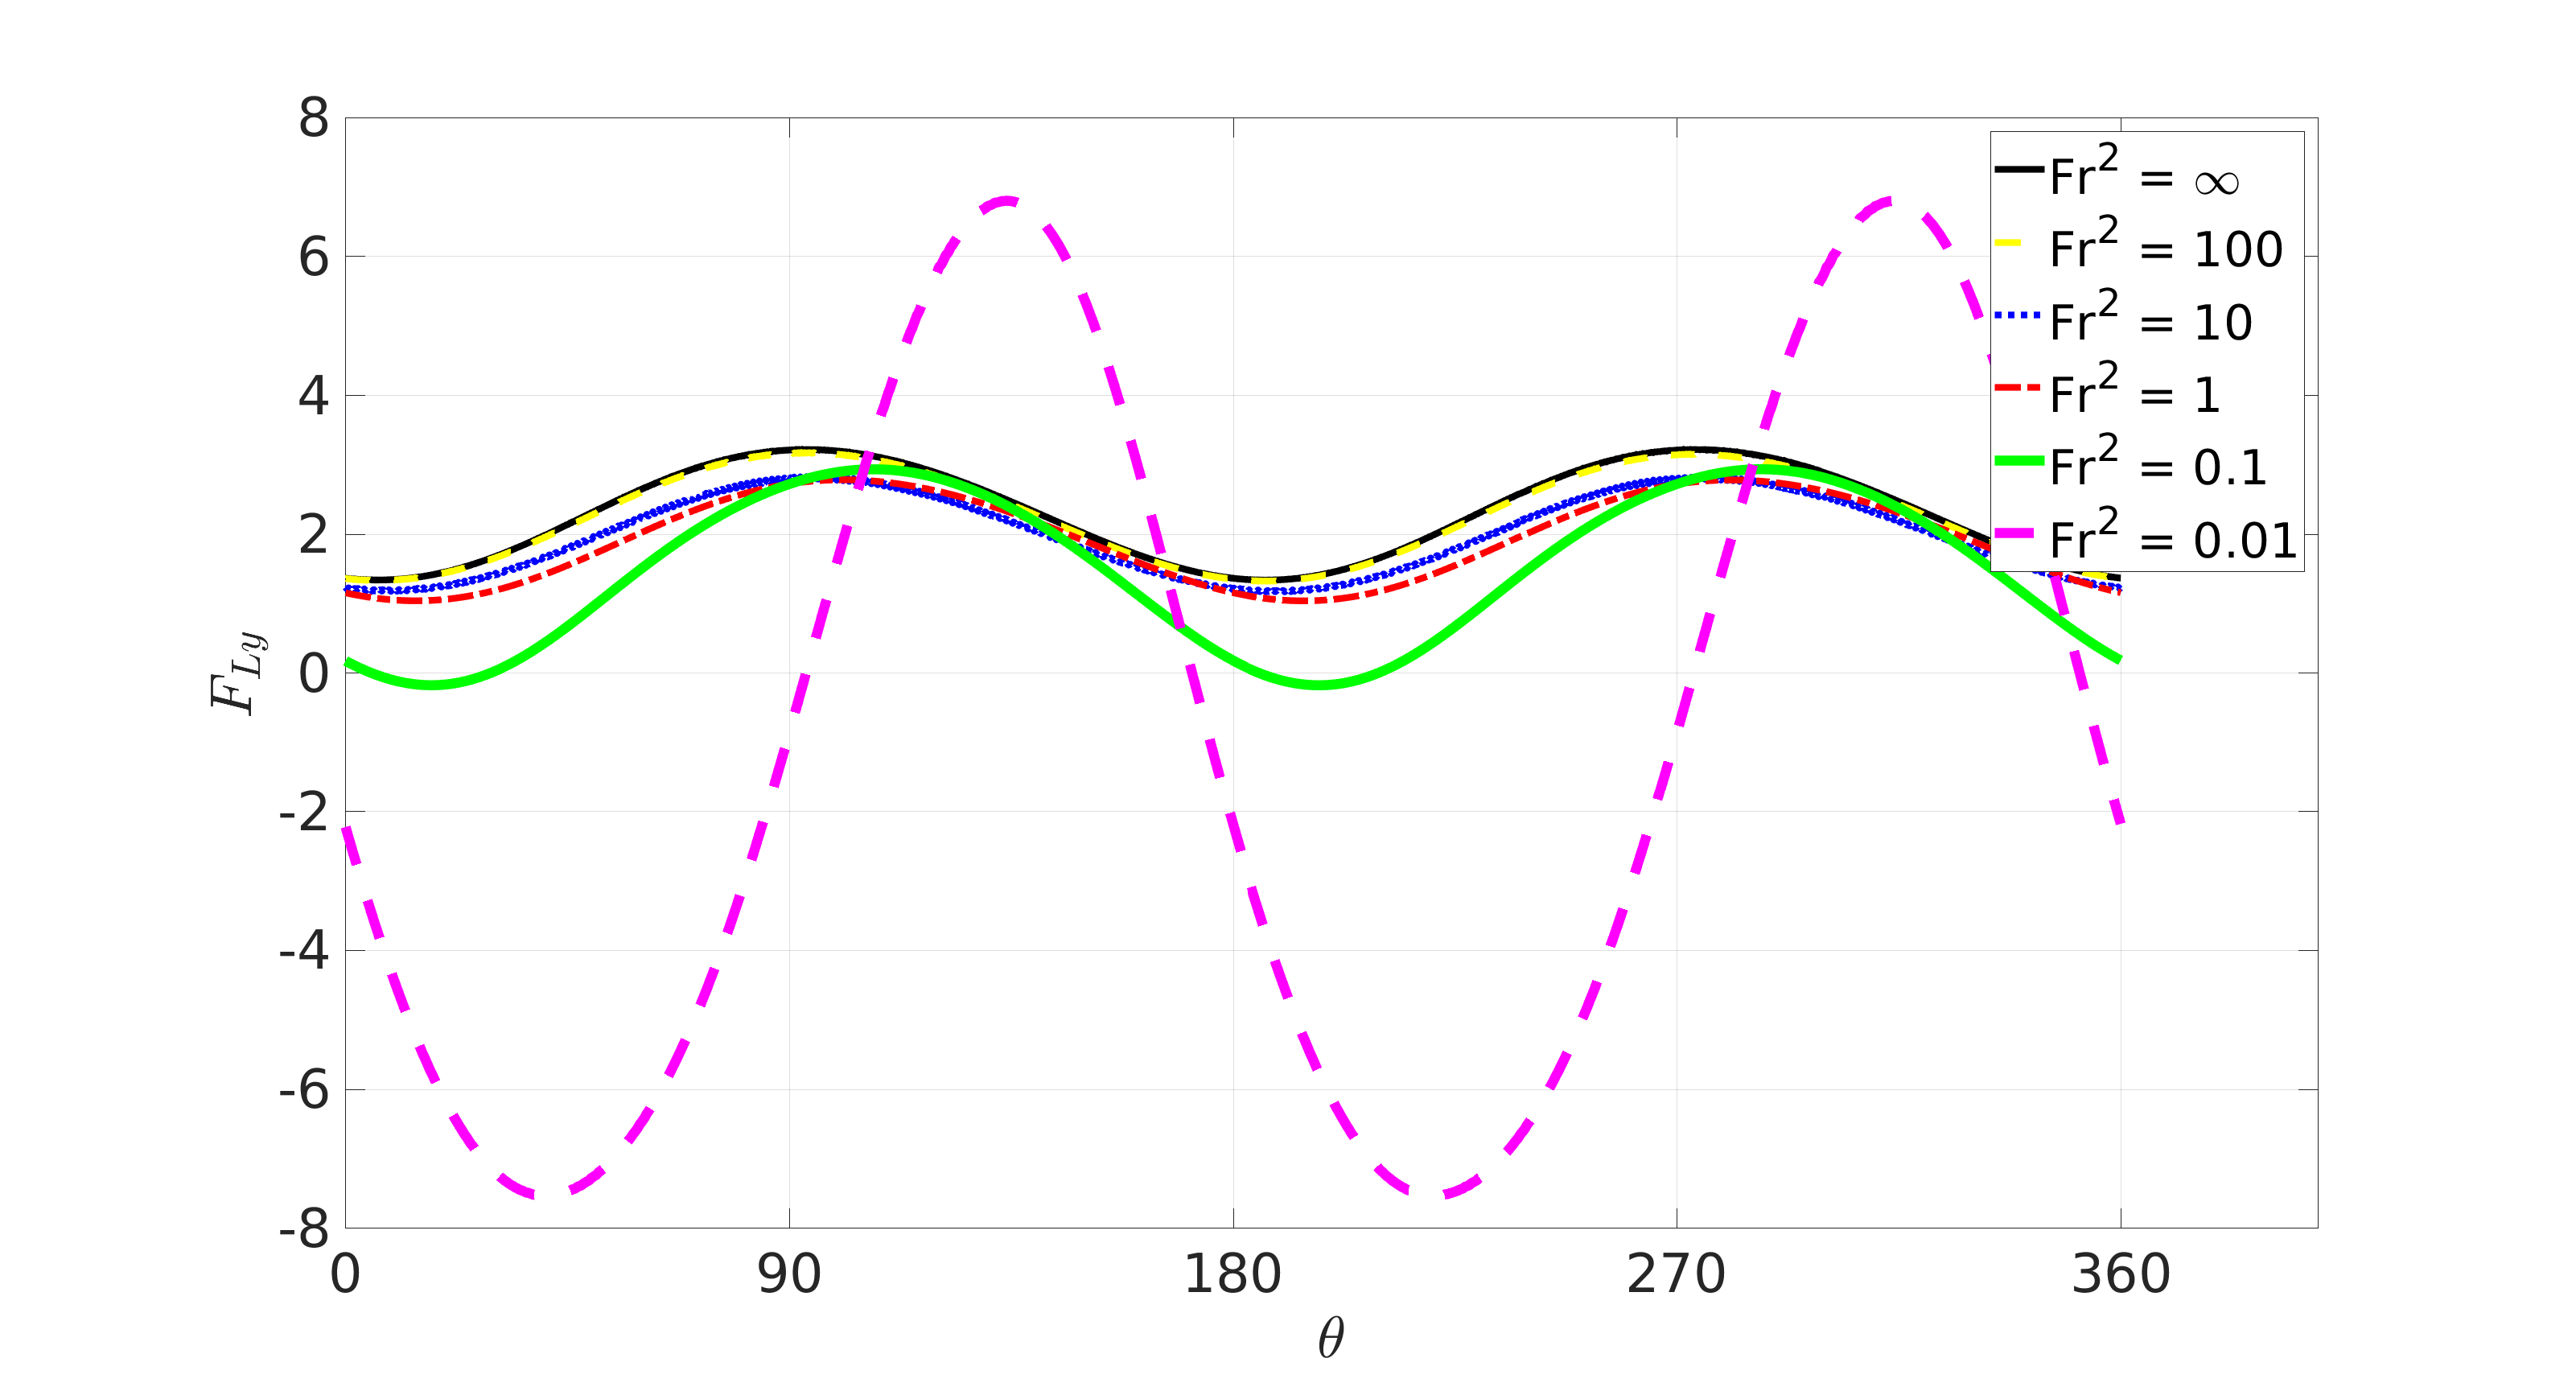
\includegraphics[width=\textwidth]{images/spinning_ellipse/palift1p5.eps}
        \caption{}
        \label{fig:palift1p5}
    \end{subfigure}
    \caption{Phase averaged drag and lift for $AR = 1.5$}
    \label{fig:pa1p5}
\end{figure}
\begin{figure}
    \centering
    \begin{subfigure}[b]{0.49\textwidth}
        \centering
        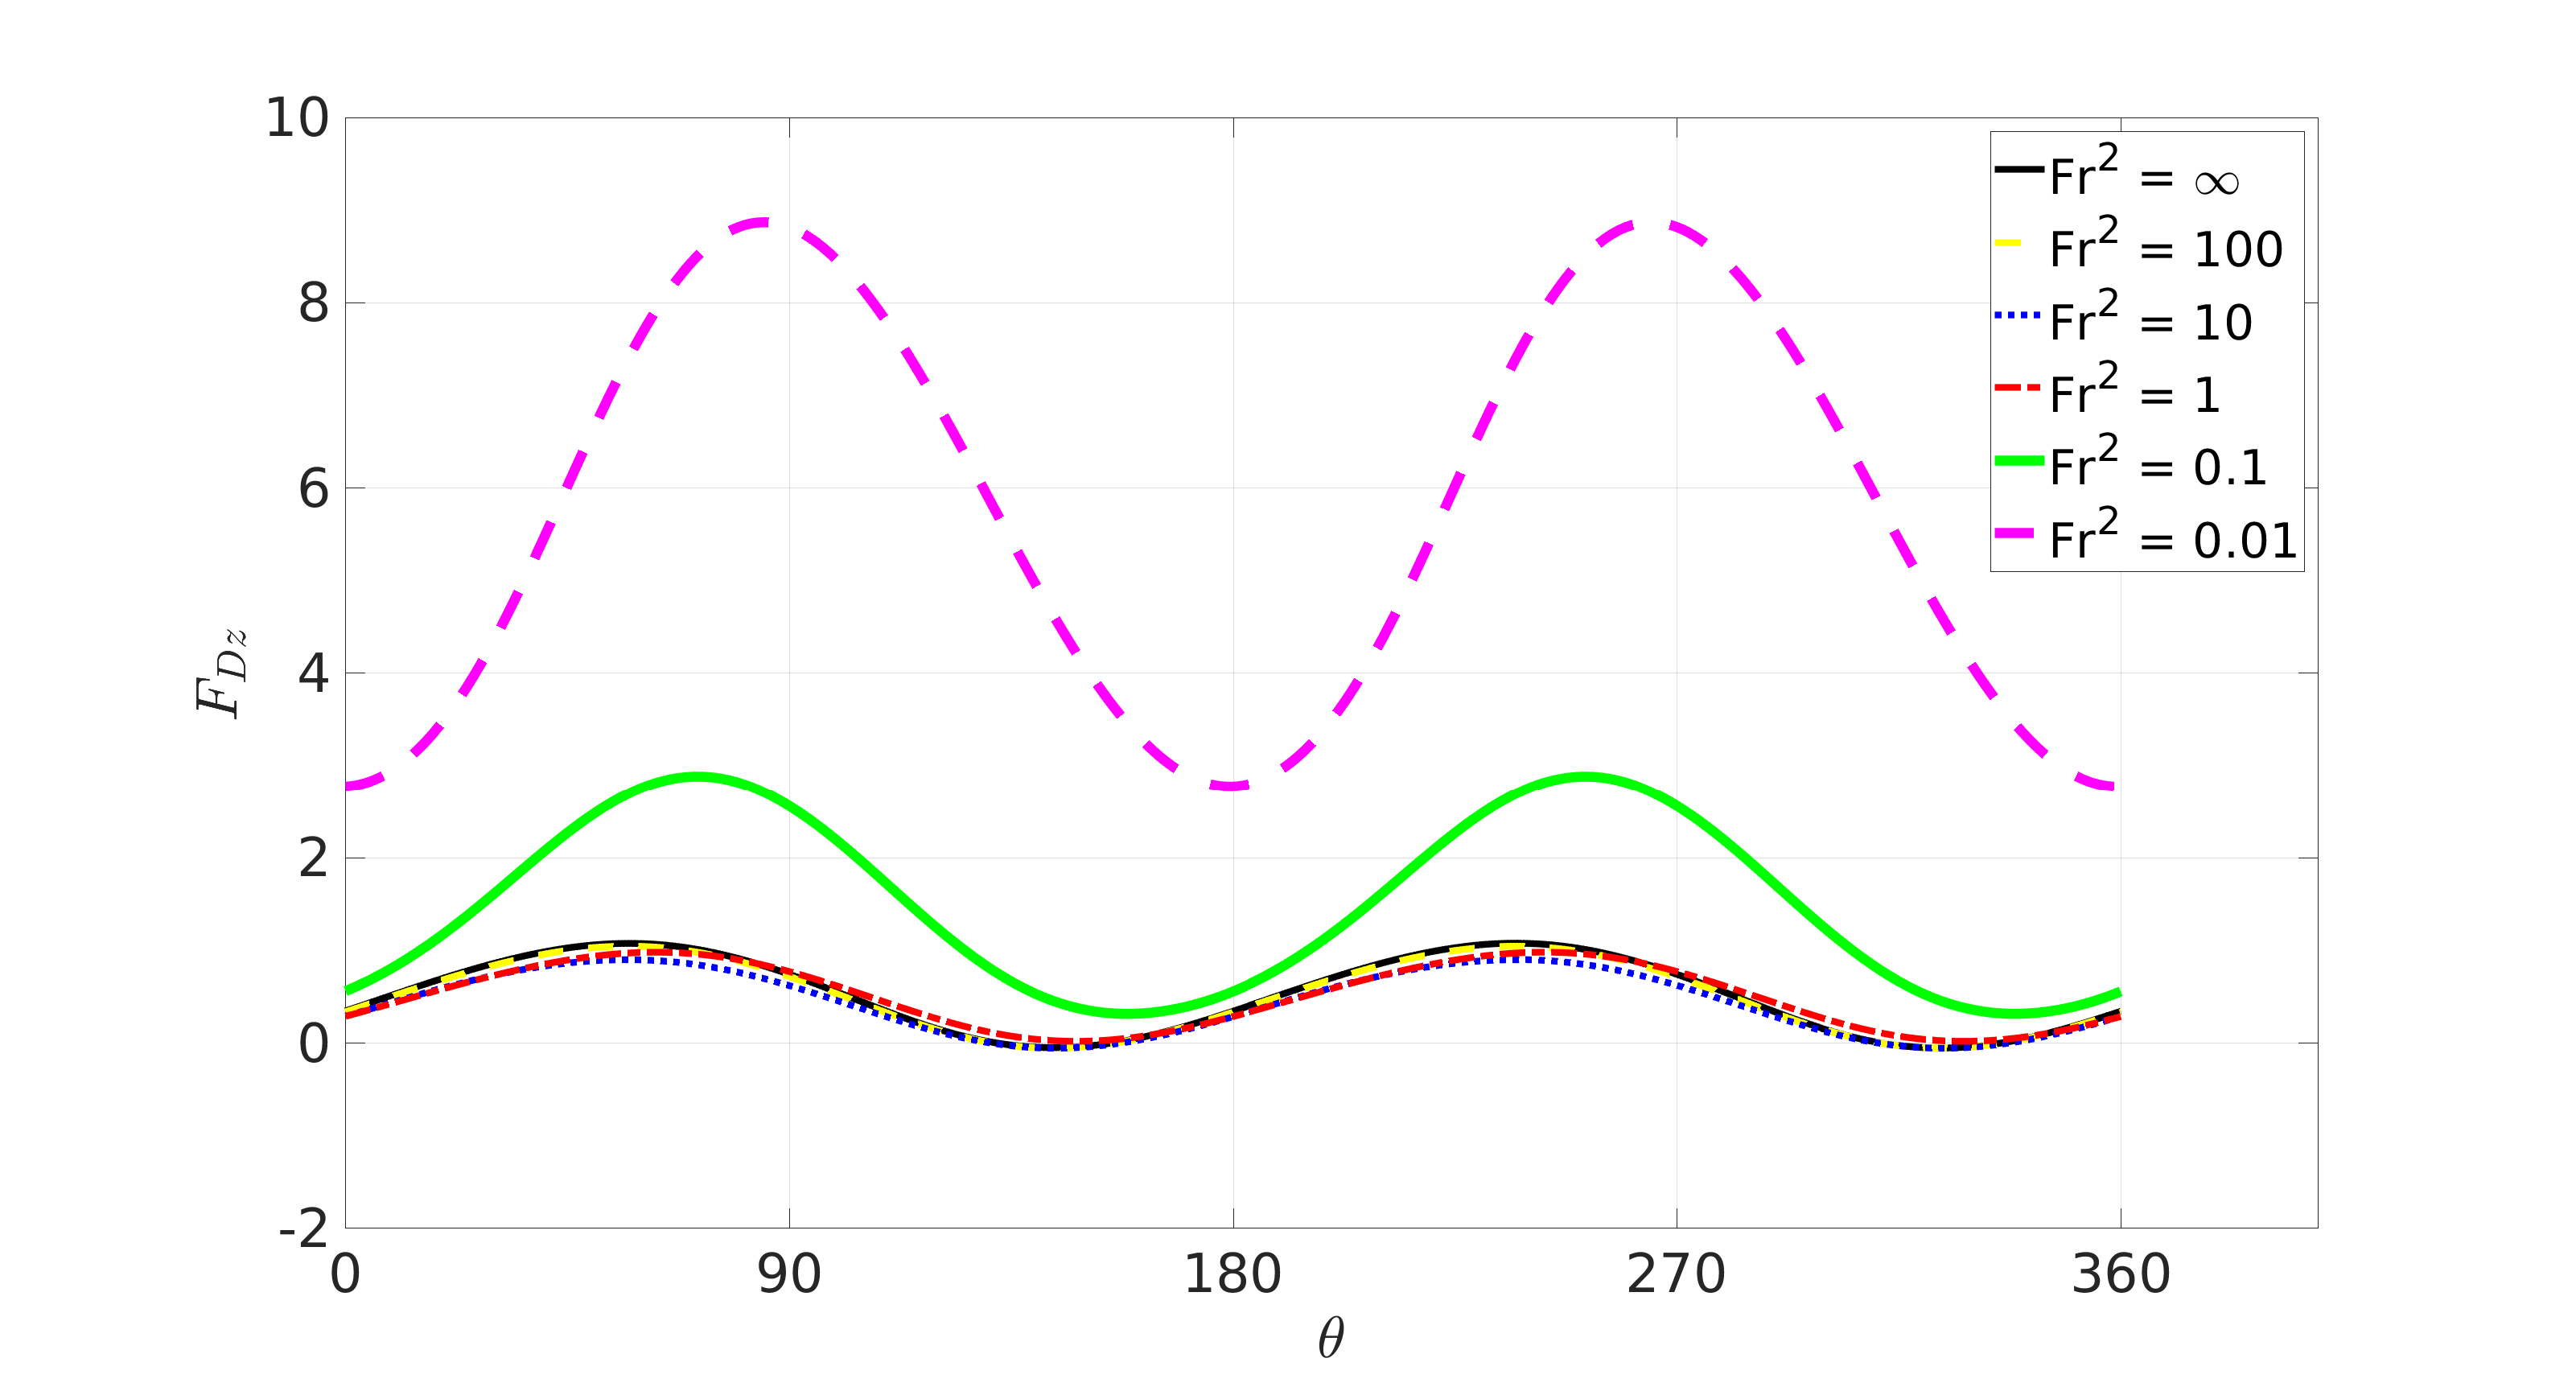
\includegraphics[width=\textwidth]{images/spinning_ellipse/padrag0p5.eps}
        \caption{}
        \label{fig:padrag0p5}
    \end{subfigure}
    \hfill
    \begin{subfigure}[b]{0.49\textwidth}
        \centering
        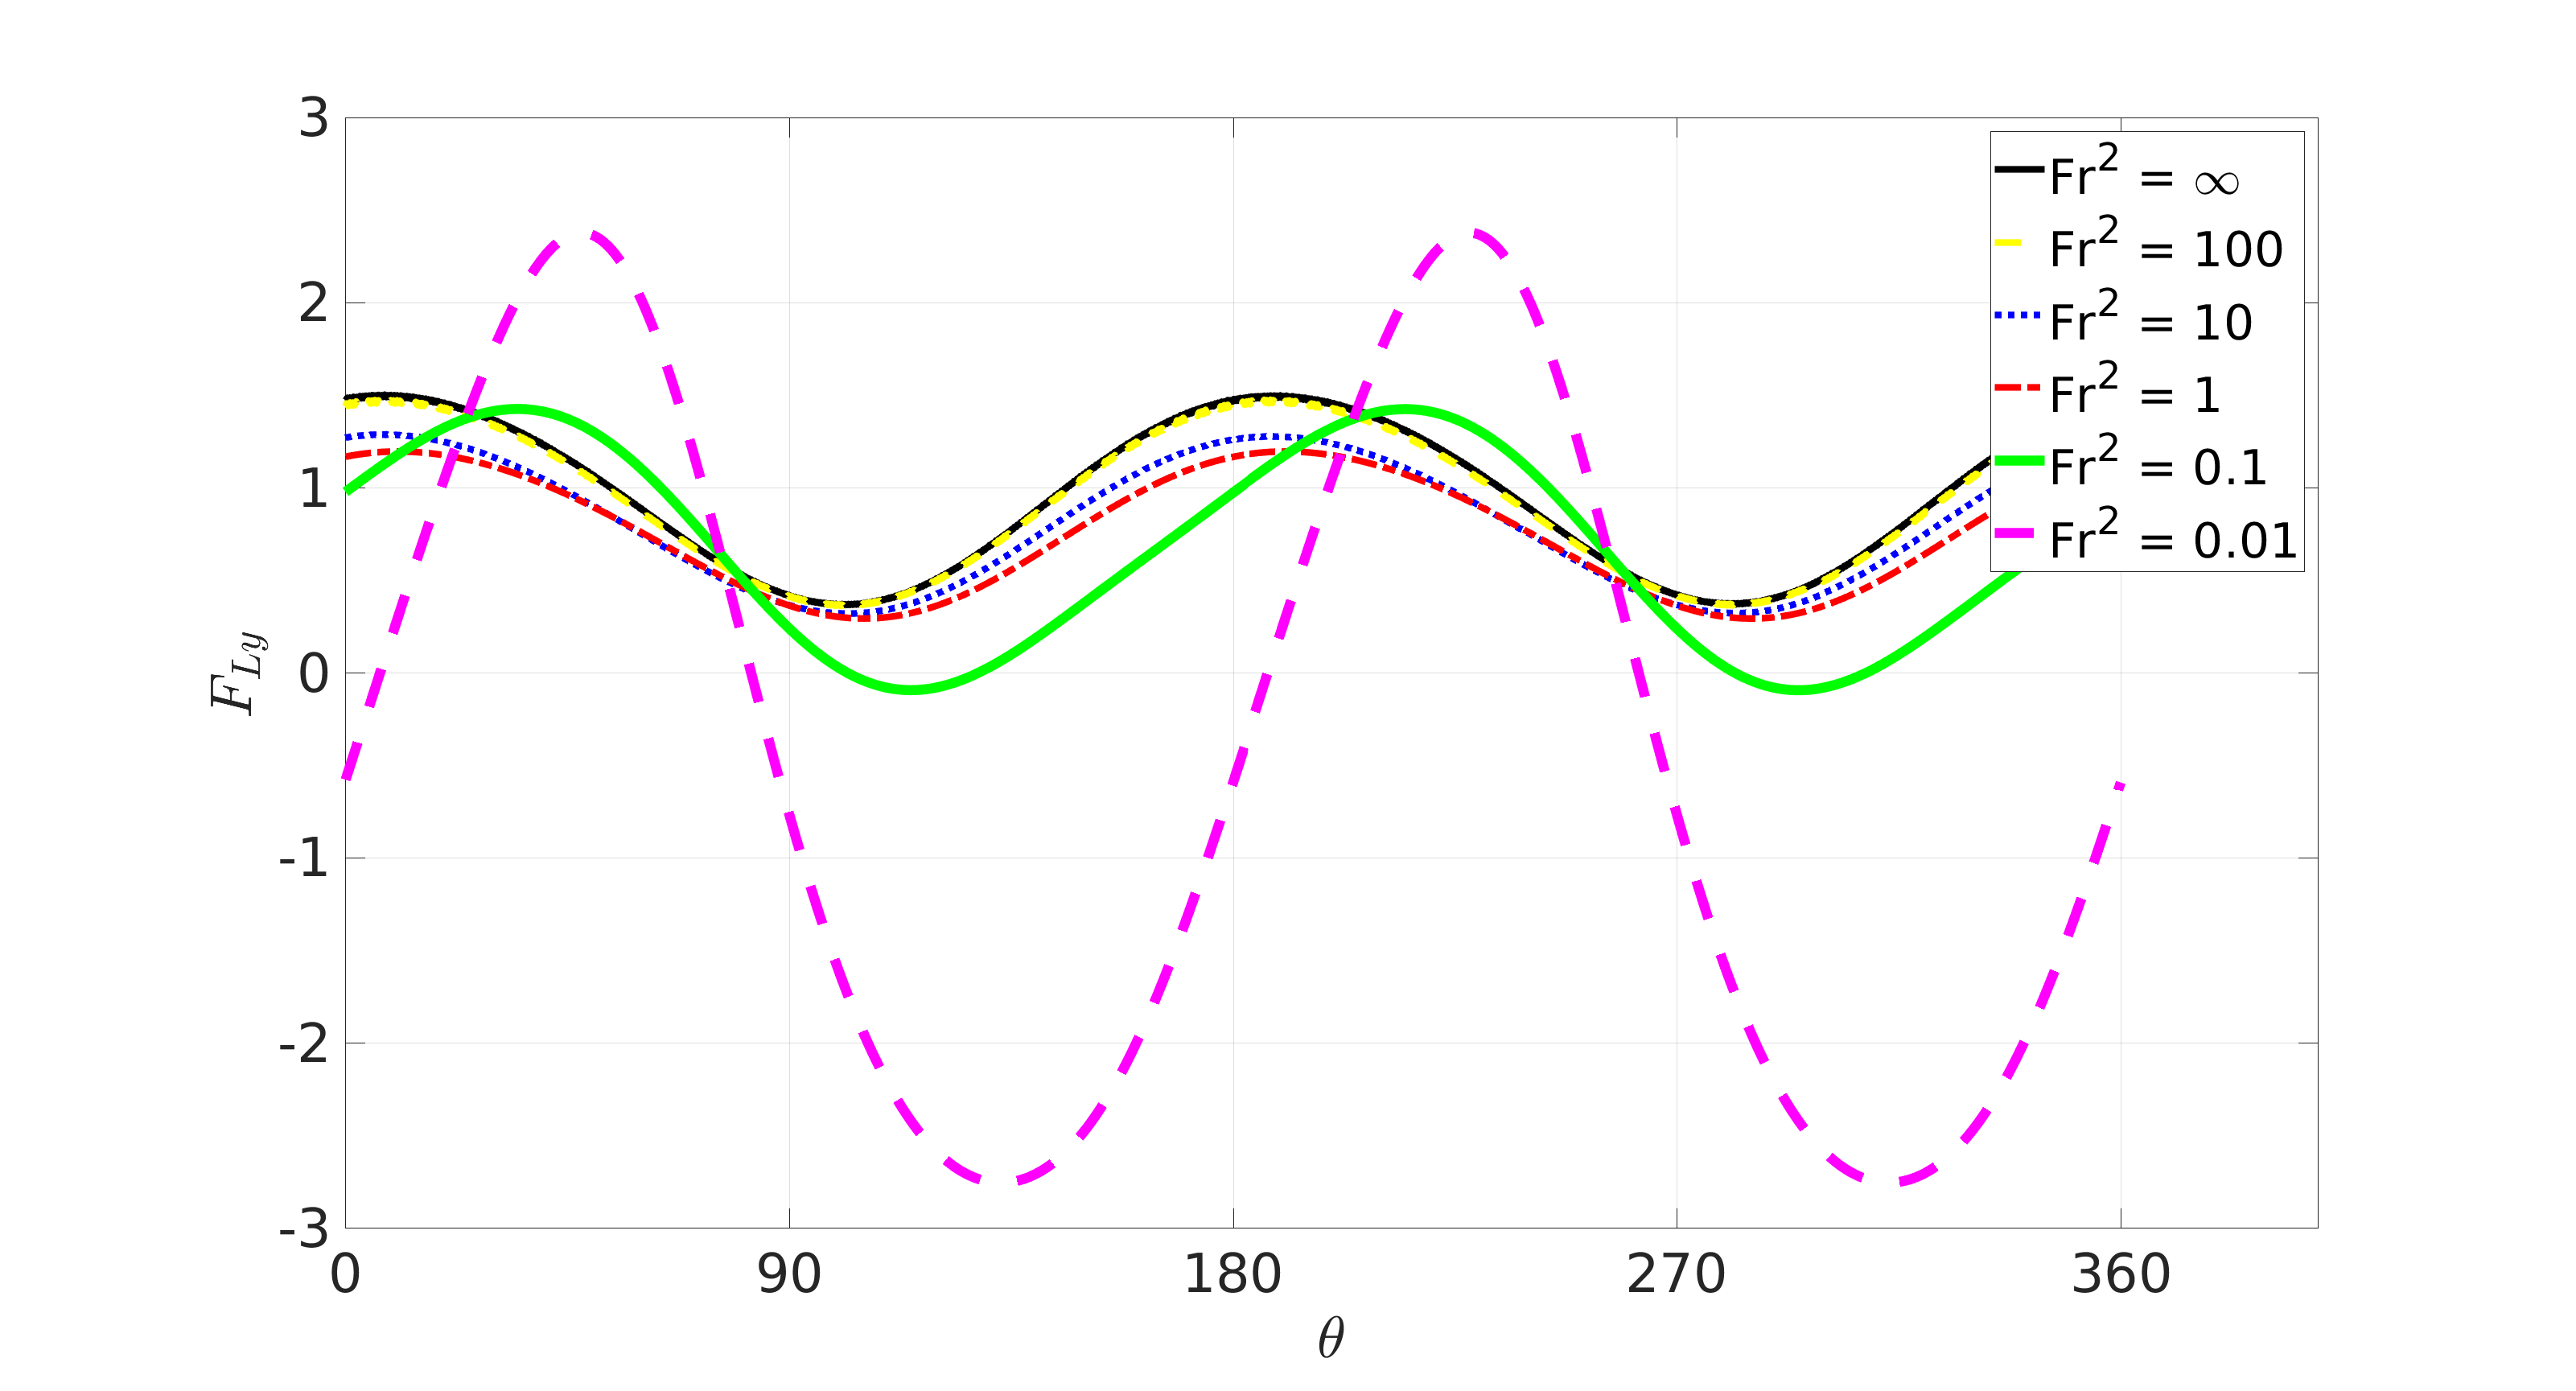
\includegraphics[width=\textwidth]{images/spinning_ellipse/palift0p5.eps}
        \caption{}
        \label{fig:palift0p5}
    \end{subfigure}
    \caption{Phase averaged drag and lift for $AR = 0.5$}
    \label{fig:pa0p5}
\end{figure}


\begin{table}
\centering
\begin{tabular}{lcc}
                 & $AR = 1.5$                 & $AR = 0.5$                \\ \hline
 $Fr^2 = \infty$ & 0.6897 [-0.6243, 1.8059]   & 0.5221 [-0.1315, 1.1414]  \\
 $Fr^2 = 100$    & 0.6702 [-0.6033, 1.7746]   & 0.5056 [-0.1329, 1.1122]  \\
 $Fr^2 = 10$     & 0.5454 [-0.4403, 1.4905]   & 0.3792 [-0.1406, 0.8591]  \\
 $Fr^2 = 1$      & 1.2342 [0.1583, 2.3695]    & 0.5097 [0.0137, 0.9888]   \\
 $Fr^2 = 0.1$    & 4.5277 [1.8280, 7.4431]    & 1.5094 [0.3125, 2.8919]   \\
 $Fr^2 = 0.01$   & 20.1590 [12.5776, 27.9980] & 5.7467 [2.7655, 8.8887]              
\end{tabular}
\caption{$F_D$}
\label{tab:fd}
\end{table}

\begin{table}
\centering
\begin{tabular}{lcc}
                 & $AR = 1.5$                 & $AR = 0.5$                 \\ \hline
 $Fr^2 = \infty$ & 2.2945 [0.8812, 4.0093]    &  0.9607 [0.0413, 1.7659]   \\
 $Fr^2 = 100$    & 2.2582 [0.8772, 3.9185]    &  0.9423 [0.2496, 1.7367]   \\
 $Fr^2 = 10$     & 1.9083 [0.8807, 3.1827]    &  0.7696 [0.2211, 1.4244]   \\
 $Fr^2 = 1$      & 1.9595 [0.9927, 2.9782]    &  0.7648 [0.2935, 1.2389]   \\
 $Fr^2 = 0.1$    & 1.4855 [-0.1808, 2.9482]   &  0.6762 [-0.1450, 1.4325]  \\
 $Fr^2 = 0.01$   & -0.9269 [-7.5654, 6.8364]  & -0.4403 [-2.7592, 2.3845]              
\end{tabular}
\caption{$F_L$}
\label{tab:fl}
\end{table}


\begin{table}
\centering
\begin{tabular}{lcc}
                 & $AR = 1.5$          & $AR = 0.5$         \\ \hline
 $Fr^2 = \infty$ & 139.7701, 319.7700  & 57.3299, 237.6899  \\
 $Fr^2 = 100$    & 140.3099, 320.8501  & 57.3299, 236.9701  \\
 $Fr^2 = 10$     & 141.2094, 321.7503  & 56.0703, 236.2502  \\
 $Fr^2 = 1$      & 153.8103, 334.1700  & 63.0899, 242.7300  \\
 $Fr^2 = 0.1$    & 159.5702, 339.5697  & 71.1906, 251.3700  \\
 $Fr^2 = 0.01$   & 176.1301, 356.1304  & 85.2299, 265.2300             
\end{tabular}
\caption{Max drag angles}
\label{tab:max_drag}
\end{table}

\begin{table}
\centering
\begin{tabular}{lcc}
                 & $AR = 1.5$          & $AR = 0.5$         \\ \hline
 $Fr^2 = \infty$ & 92.6103, 271.3496   & 8.0099, 189.6304   \\
 $Fr^2 = 100$    & 92.4299, 273.6899   & 8.0099, 187.6501   \\
 $Fr^2 = 10$     & 93.3300, 274.7704   & 6.5699, 187.6500   \\
 $Fr^2 = 1$      & 99.9902, 280.7099   & 10.3505, 190.5300  \\
 $Fr^2 = 0.1$    & 107.3702, 287.1896  & 35.0101, 214.8302  \\
 $Fr^2 = 0.01$   & 134.0096, 314.0104  & 47.6098, 227.6099             
\end{tabular}
\caption{Max lift angles}
\label{tab:max_lift}
\end{table}
\begin{figure}
    \centering
    \begin{subfigure}[b]{0.25\textwidth}
        \centering
        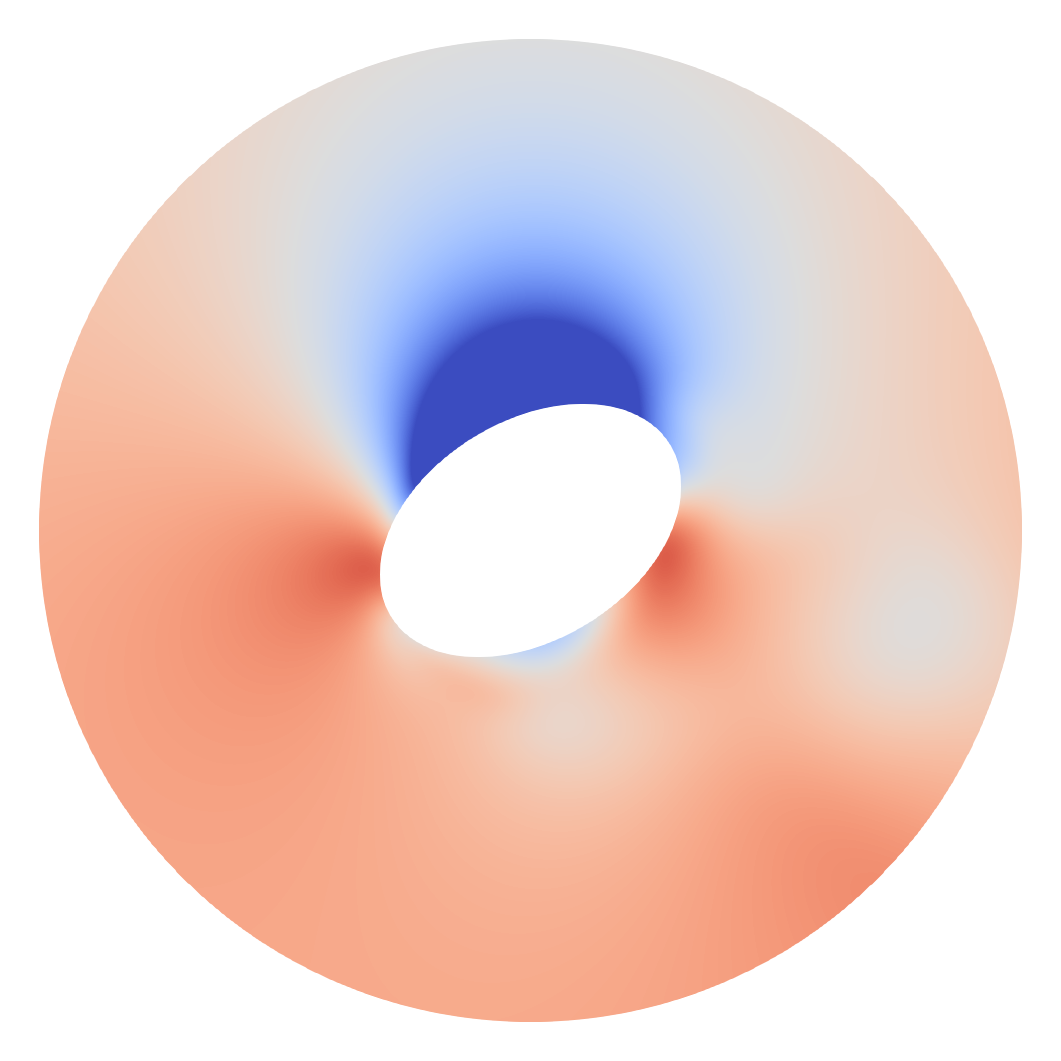
\includegraphics[width=\textwidth]{images/spinning_ellipse/par1p5fsinf.png}
        \caption{$Fr^2 = \infty$}
        \label{fig:par1p5fsinf}
    \end{subfigure}
    \hfill
    \begin{subfigure}[b]{0.25\textwidth}
        \centering
        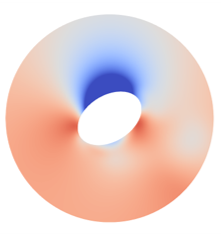
\includegraphics[width=\textwidth]{images/spinning_ellipse/par1p5fs100.png}
        \caption{$Fr^2 = 100$}
        \label{fig:par1p5fs100}
    \end{subfigure}
    \hfill
    \begin{subfigure}[b]{0.25\textwidth}
        \centering
        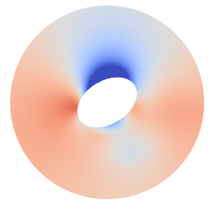
\includegraphics[width=\textwidth]{images/spinning_ellipse/par1p5fs10.png}
        \caption{$Fr^2 = 10$}
        \label{fig:par1p5fs10}
    \end{subfigure}
    
    \begin{subfigure}[b]{0.25\textwidth}
        \centering
        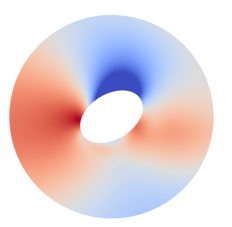
\includegraphics[width=\textwidth]{images/spinning_ellipse/par1p5fs1.png}
        \caption{$Fr^2 = 1$}
        \label{fig:par1p5fs1}
    \end{subfigure}
    \hfill
    \begin{subfigure}[b]{0.25\textwidth}
        \centering
        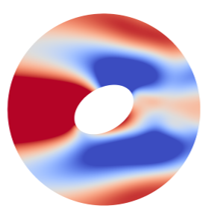
\includegraphics[width=\textwidth]{images/spinning_ellipse/par1p5fs0p1.png}
        \caption{$Fr^2 = 0.1$}
        \label{fig:par1p5fs0p1}
    \end{subfigure}
    \hfill
    \begin{subfigure}[b]{0.25\textwidth}
        \centering
        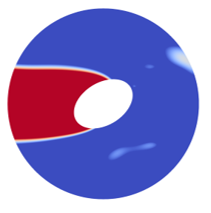
\includegraphics[width=\textwidth]{images/spinning_ellipse/par1p5fs0p01.png}
        \caption{$Fr^2 = 0.01$}
        \label{fig:par1p5fs0p01}
    \end{subfigure}
    
    \begin{subfigure}[b]{0.25\textwidth}
        \centering
        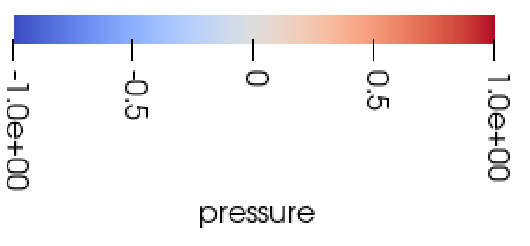
\includegraphics[width=\textwidth]{images/spinning_ellipse/p_scale.png}
        \caption*{}
    \end{subfigure}
    
    \caption{A comparison of the pressure fields for spinning ellipse where $AR = 1.5$}
    \label{fig:ar1p5_pressure}
\end{figure}

\begin{figure}
    \centering
    \begin{subfigure}[b]{0.25\textwidth}
        \centering
        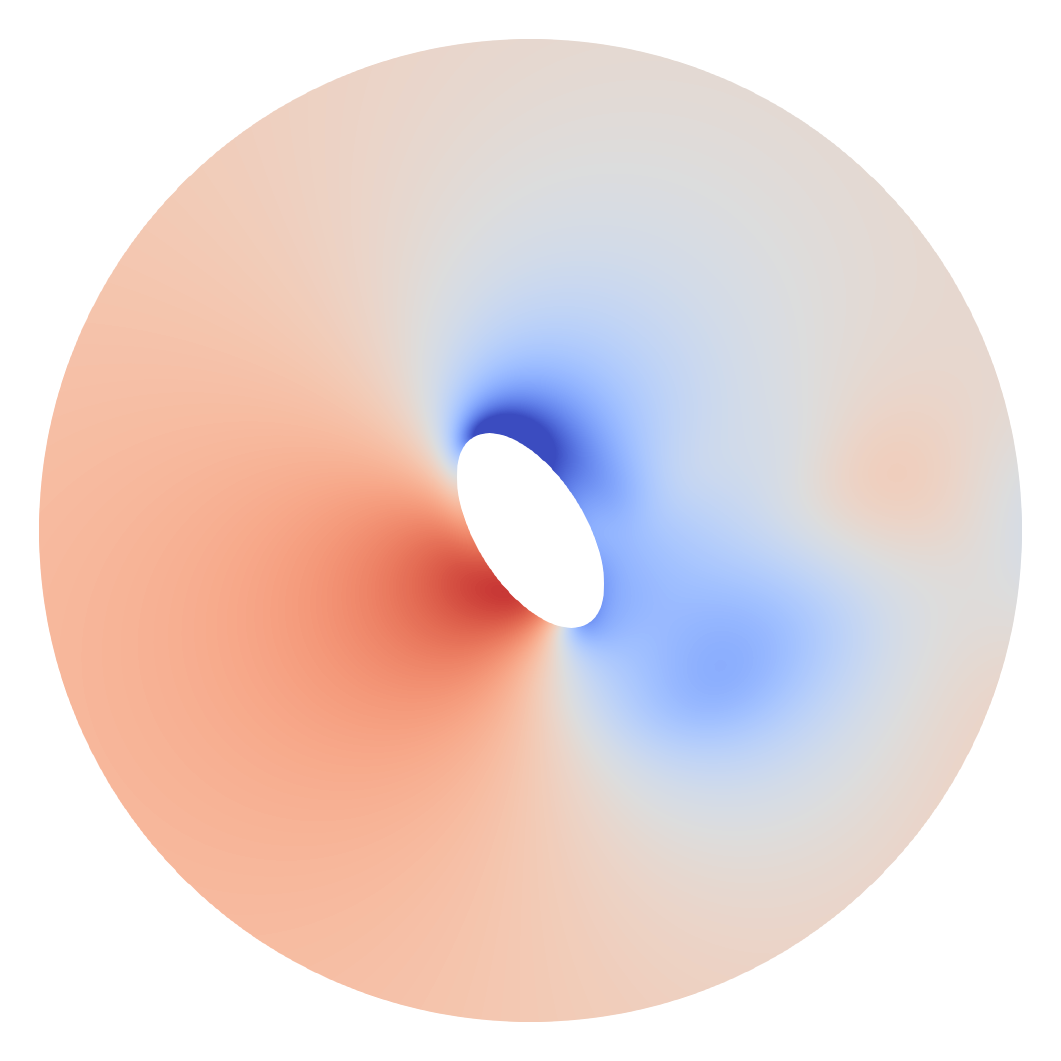
\includegraphics[width=\textwidth]{images/spinning_ellipse/par0p5fsinf.png}
        \caption{$Fr^2 = \infty$}
        \label{fig:par0p5fsinf}
    \end{subfigure}
    \hfill
    \begin{subfigure}[b]{0.25\textwidth}
        \centering
        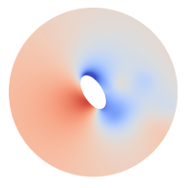
\includegraphics[width=\textwidth]{images/spinning_ellipse/par0p5fs100.png}
        \caption{$Fr^2 = 100$}
        \label{fig:par0p5fs100}
    \end{subfigure}
    \hfill
    \begin{subfigure}[b]{0.25\textwidth}
        \centering
        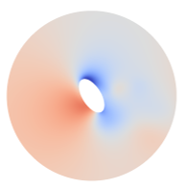
\includegraphics[width=\textwidth]{images/spinning_ellipse/par0p5fs10.png}
        \caption{$Fr^2 = 10$}
        \label{fig:par0p5fs10}
    \end{subfigure}
    
    \begin{subfigure}[b]{0.25\textwidth}
        \centering
        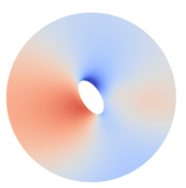
\includegraphics[width=\textwidth]{images/spinning_ellipse/par0p5fs1.png}
        \caption{$Fr^2 = 1$}
        \label{fig:par0p5fs1}
    \end{subfigure}
    \hfill
    \begin{subfigure}[b]{0.25\textwidth}
        \centering
        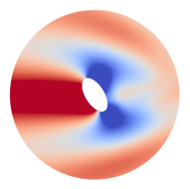
\includegraphics[width=\textwidth]{images/spinning_ellipse/par0p5fs0p1.png}
        \caption{$Fr^2 = 0.1$}
        \label{fig:par0p5fs0p1}
    \end{subfigure}
    \hfill
    \begin{subfigure}[b]{0.25\textwidth}
        \centering
        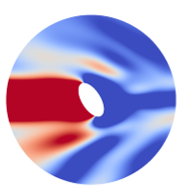
\includegraphics[width=\textwidth]{images/spinning_ellipse/par0p5fs0p01.png}
        \caption{$Fr^2 = 0.01$}
        \label{fig:par0p5fs0p01}
    \end{subfigure}
    
    \begin{subfigure}[b]{0.25\textwidth}
        \centering
        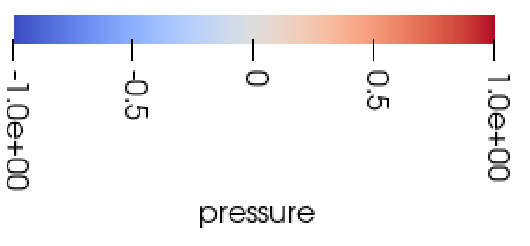
\includegraphics[width=\textwidth]{images/spinning_ellipse/p_scale.png}
        \caption*{}
    \end{subfigure}
    
    \caption{A comparison of the pressure fields for spinning ellipse where $AR = 0.5$}
    \label{fig:ar0p5_pressure}
\end{figure}
\clearpage
\subsubsection{Flow structures}
Figures \ref{fig:ar1p5 y-vel} and \ref{fig:ar0p5 y-vel} show similar flow patterns observed in the circular cases. The gravity waves propagate most strongly at around $Fr^2 = 1$. The plots also show a flow regime transition around $Fr^2 = 1$. We observe that with both aspect ratios, just like in the results from literature \cite{ortiz-tarin_stratified_2019}, there are circular patterns in the y-velocity around the body. Just like in the circular cases, we observe a transition in the flow type around $Fr^2 = 1$. At $Fr^2$, we see the gravity waves breaking up the paths of vortices.  Although the flow structures look the same for both aspect ratios, we observe that the magnitudes in the case of $AR = 1.5$ are larger. This is because even though $\Rey$ is the same based on our methodology, the \textit{effective} $\Rey$ increases with aspect ratio due to the larger of momentum effects from the larger body. An interesting insight is how little effect the aspect ratio has on the flow structures. Higher aspect ratio bodies show slightly larger magnitudes in the y-velocity plots, but the structures of the features look the same. We observed periodic semi-circular patterns y-velocity fields at $Fr^2 = 1, 0.1$ like in literature \cite{ortiz-tarin_stratified_2019}. Figures \ref{fig:schlerienar1p5} and \ref{fig:schlerienar0p5} give us schlerien plots of the spinning ellipses. ANTON NEEDS TO LOOK MORE AT TRANSITIONS
\begin{figure}
    \centering
    \begin{subfigure}[b]{0.32\textwidth}
        \centering
        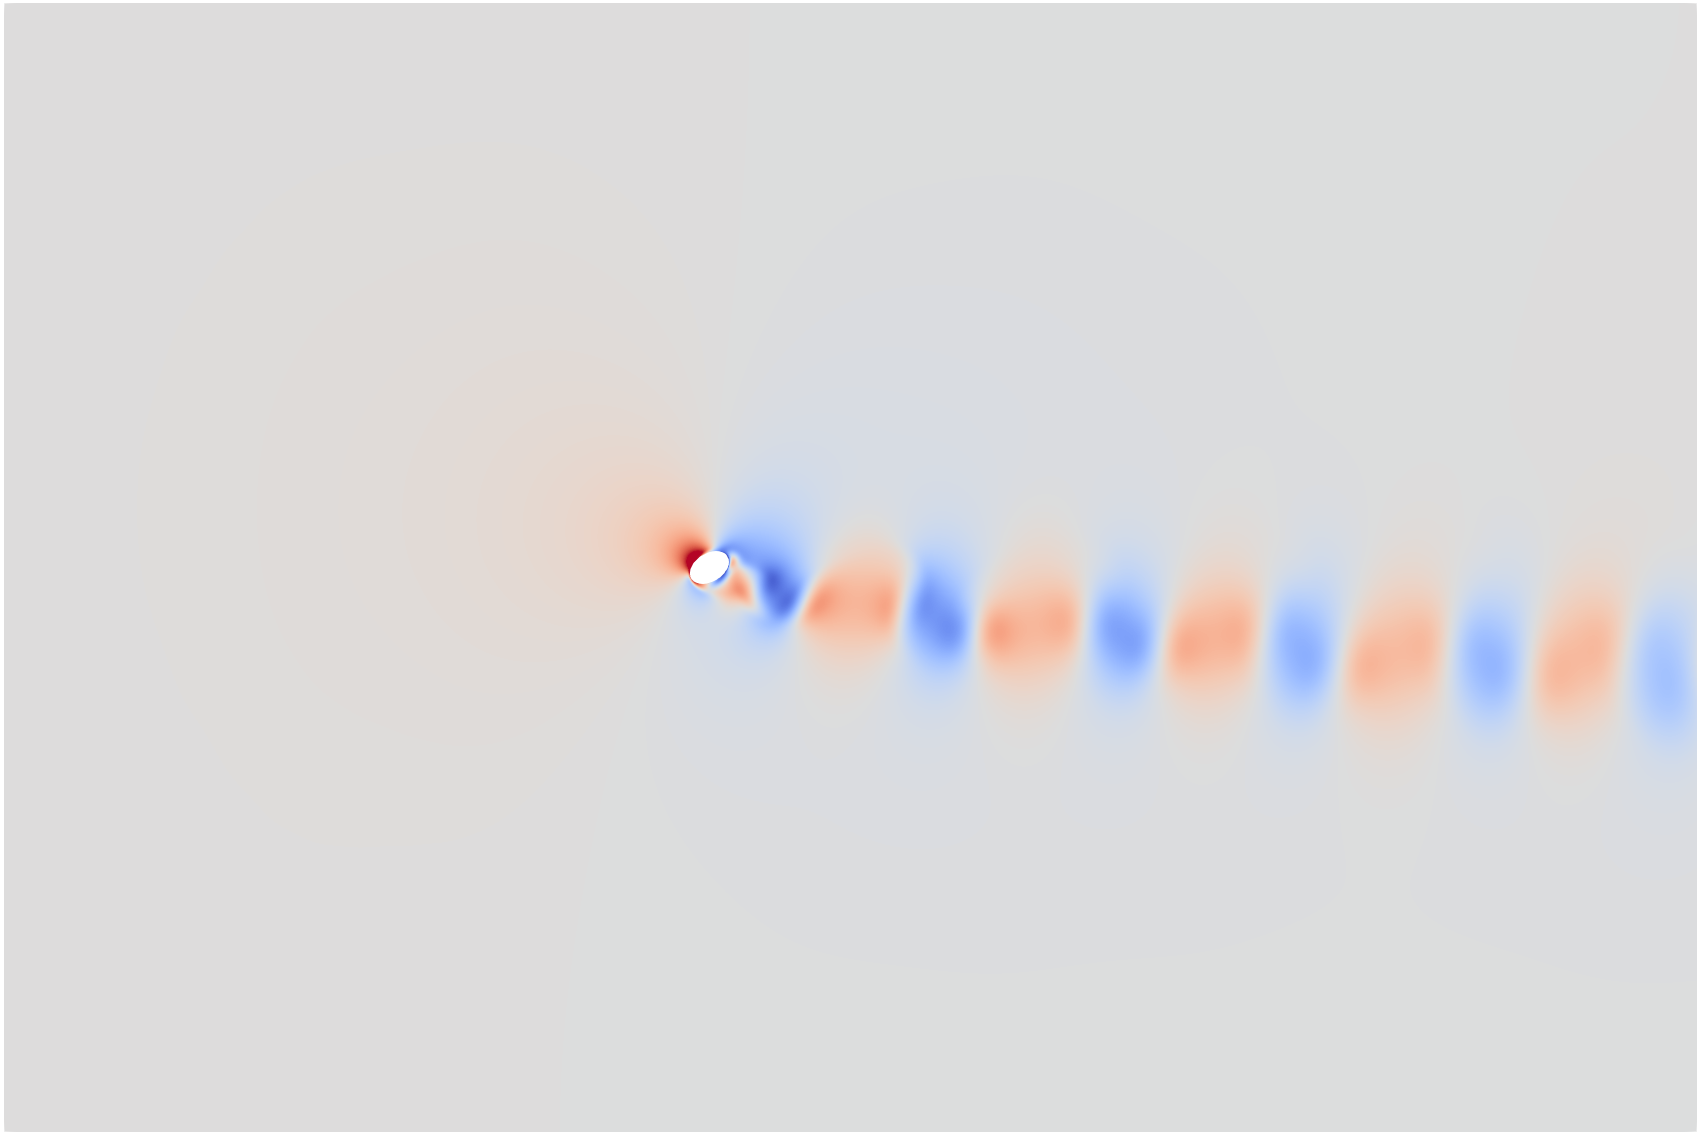
\includegraphics[width=\textwidth]{images/spinning_ellipse/ar1p5fsinf.png}
        \caption{$Fr^2 = \infty$}
        \label{fig:ar1p5fsinf}
    \end{subfigure}
    \hfill
    \begin{subfigure}[b]{0.32\textwidth}
        \centering
        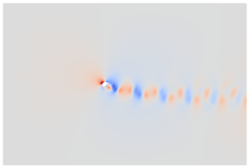
\includegraphics[width=\textwidth]{images/spinning_ellipse/ar1p5fr10.png}
        \caption{$Fr^2 = 100$}
        \label{fig:ar1p5fr10}
    \end{subfigure}
    \hfill
    \begin{subfigure}[b]{0.32\textwidth}
        \centering
        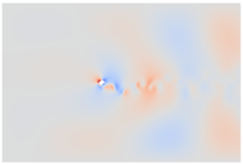
\includegraphics[width=\textwidth]{images/spinning_ellipse/ar1p5fr3.png}
        \caption{$Fr^2 = 10$}
        \label{fig:ar1p5fr3}
    \end{subfigure}
    
    \begin{subfigure}[b]{0.32\textwidth}
        \centering
        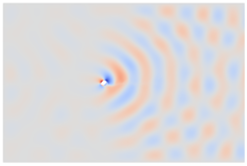
\includegraphics[width=\textwidth]{images/spinning_ellipse/ar1p5fr1.png}
        \caption{$Fr^2 = 1$}
        \label{fig:ar1p5fr1}
    \end{subfigure}
    \hfill
    \begin{subfigure}[b]{0.32\textwidth}
        \centering
        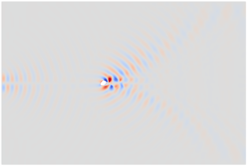
\includegraphics[width=\textwidth]{images/spinning_ellipse/ar1p5fr0p3.png}
        \caption{$Fr^2 = 0.1$}
        \label{fig:ar1p5fr0p3}
    \end{subfigure}
    \hfill
    \begin{subfigure}[b]{0.32\textwidth}
        \centering
        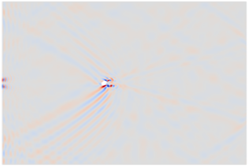
\includegraphics[width=\textwidth]{images/spinning_ellipse/ar1p5fr0p1.png}
        \caption{$Fr^2 = 0.01$}
        \label{fig:ar1p5fr0p1}
    \end{subfigure}
    
    \begin{subfigure}[b]{0.32\textwidth}
        \centering
        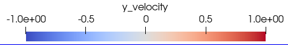
\includegraphics[width=\textwidth]{images/spinning_ellipse/scale1.png}
        \caption*{}
    \end{subfigure}
    
    \caption{A comparison of the y-velocity fields for spinning ellipse where $AR = 1.5$}
    \label{fig:ar1p5 y-vel}
\end{figure}

\begin{figure}
    \centering
    \begin{subfigure}[b]{0.32\textwidth}
        \centering
        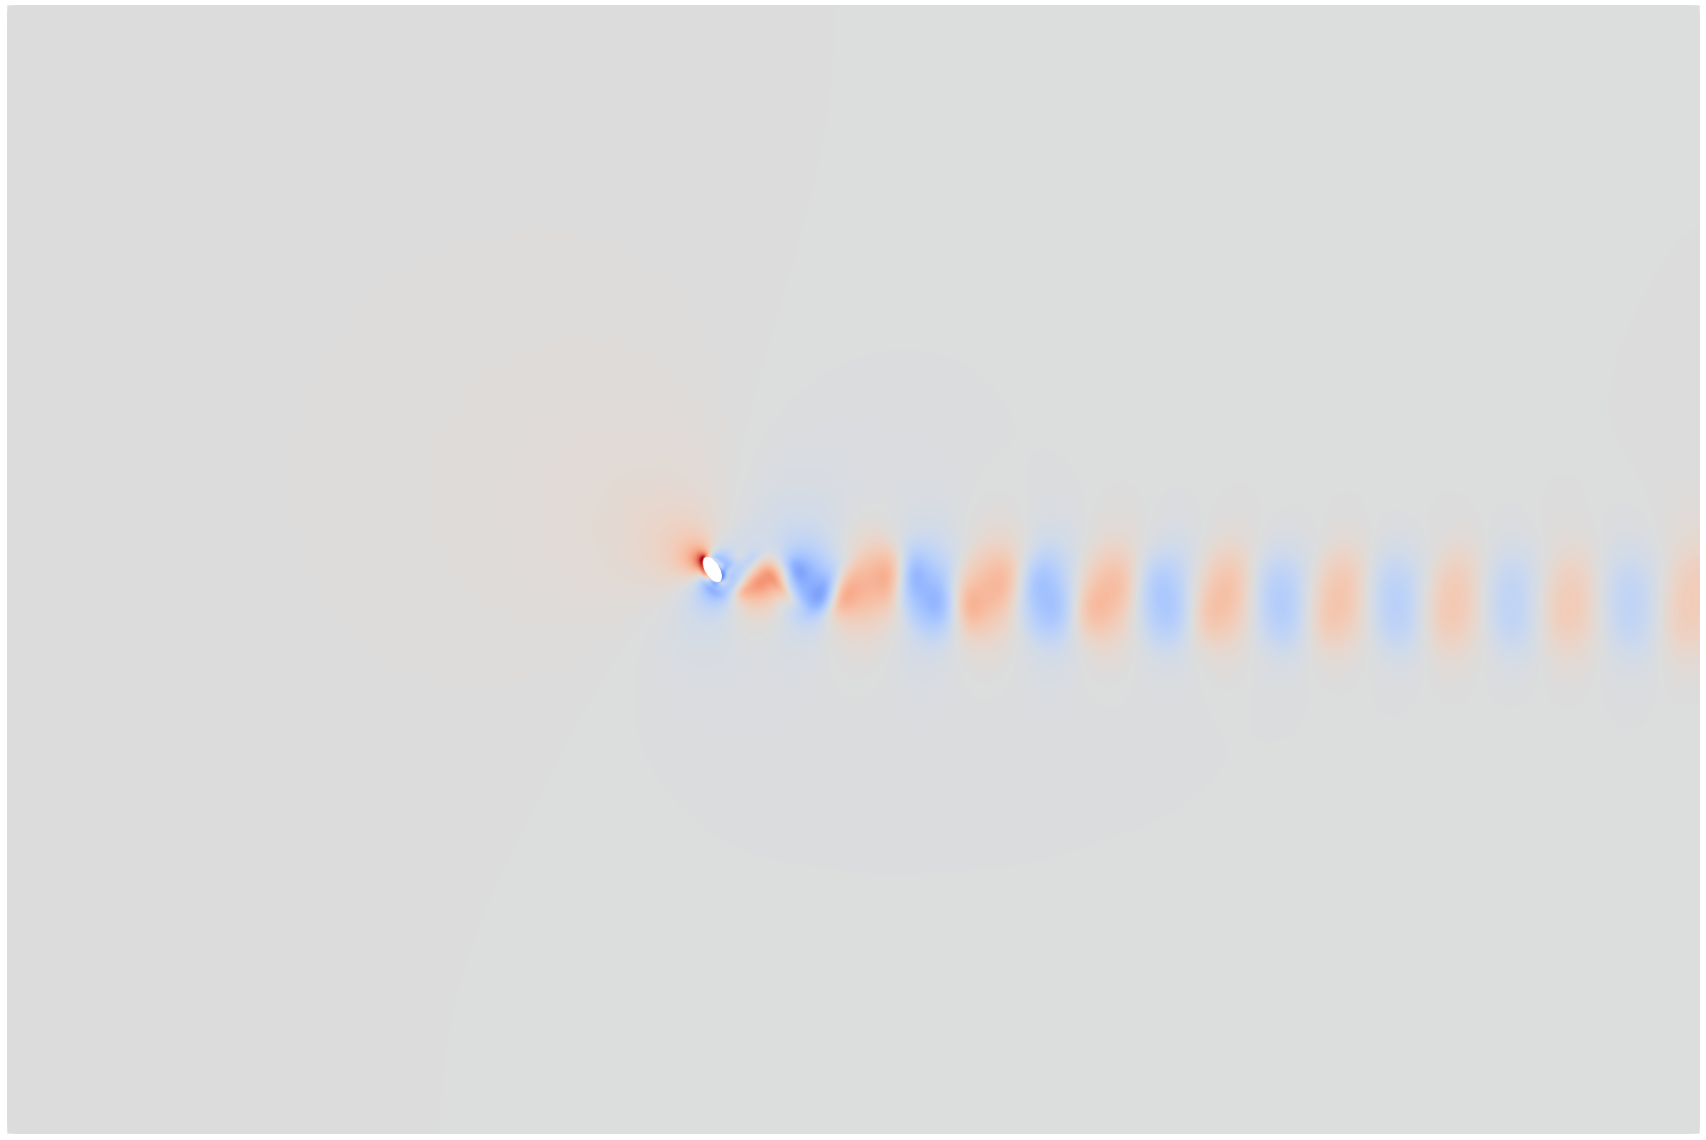
\includegraphics[width=\textwidth]{images/spinning_ellipse/ar0p5fsinf.png}
        \caption{$Fr^2 = \infty$}
        \label{fig:ar0p5fsinf}
    \end{subfigure}
    \hfill
    \begin{subfigure}[b]{0.32\textwidth}
        \centering
        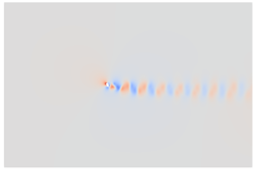
\includegraphics[width=\textwidth]{images/spinning_ellipse/ar0p5fr10.png}
        \caption{$Fr^2 = 100$}
        \label{fig:ar0p5fr10}
    \end{subfigure}
    \hfill
    \begin{subfigure}[b]{0.32\textwidth}
        \centering
        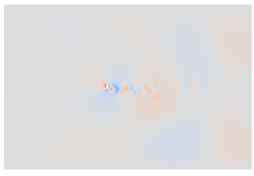
\includegraphics[width=\textwidth]{images/spinning_ellipse/ar0p5fr3.png}
        \caption{$Fr^2 = 10$}
        \label{fig:ar0p5fr3}
    \end{subfigure}
    
    \begin{subfigure}[b]{0.32\textwidth}
        \centering
        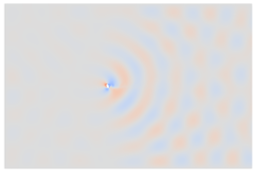
\includegraphics[width=\textwidth]{images/spinning_ellipse/ar0p5fr1.png}
        \caption{$Fr^2 = 1$}
        \label{fig:ar0p5fr1}
    \end{subfigure}
    \hfill
    \begin{subfigure}[b]{0.32\textwidth}
        \centering
        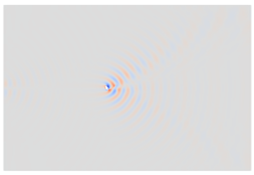
\includegraphics[width=\textwidth]{images/spinning_ellipse/ar0p5fr0p3.png}
        \caption{$Fr^2 = 0.1$}
        \label{fig:ar0p5fr0p3}
    \end{subfigure}
    \hfill
    \begin{subfigure}[b]{0.32\textwidth}
        \centering
        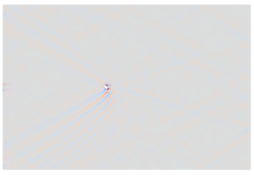
\includegraphics[width=\textwidth]{images/spinning_ellipse/ar0p5fr0p1.png}
        \caption{$Fr^2 = 0.01$}
        \label{fig:ar0p5fr0p1}
    \end{subfigure}
    
    \begin{subfigure}[b]{0.32\textwidth}
        \centering
        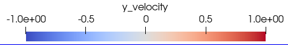
\includegraphics[width=\textwidth]{images/spinning_ellipse/scale1.png}
        \caption*{}
    \end{subfigure}
    
    \caption{A comparison of the y-velocity fields for spinning ellipse where $AR = 0.5$}
    \label{fig:ar0p5 y-vel}
\end{figure}
\begin{figure}
    \centering
    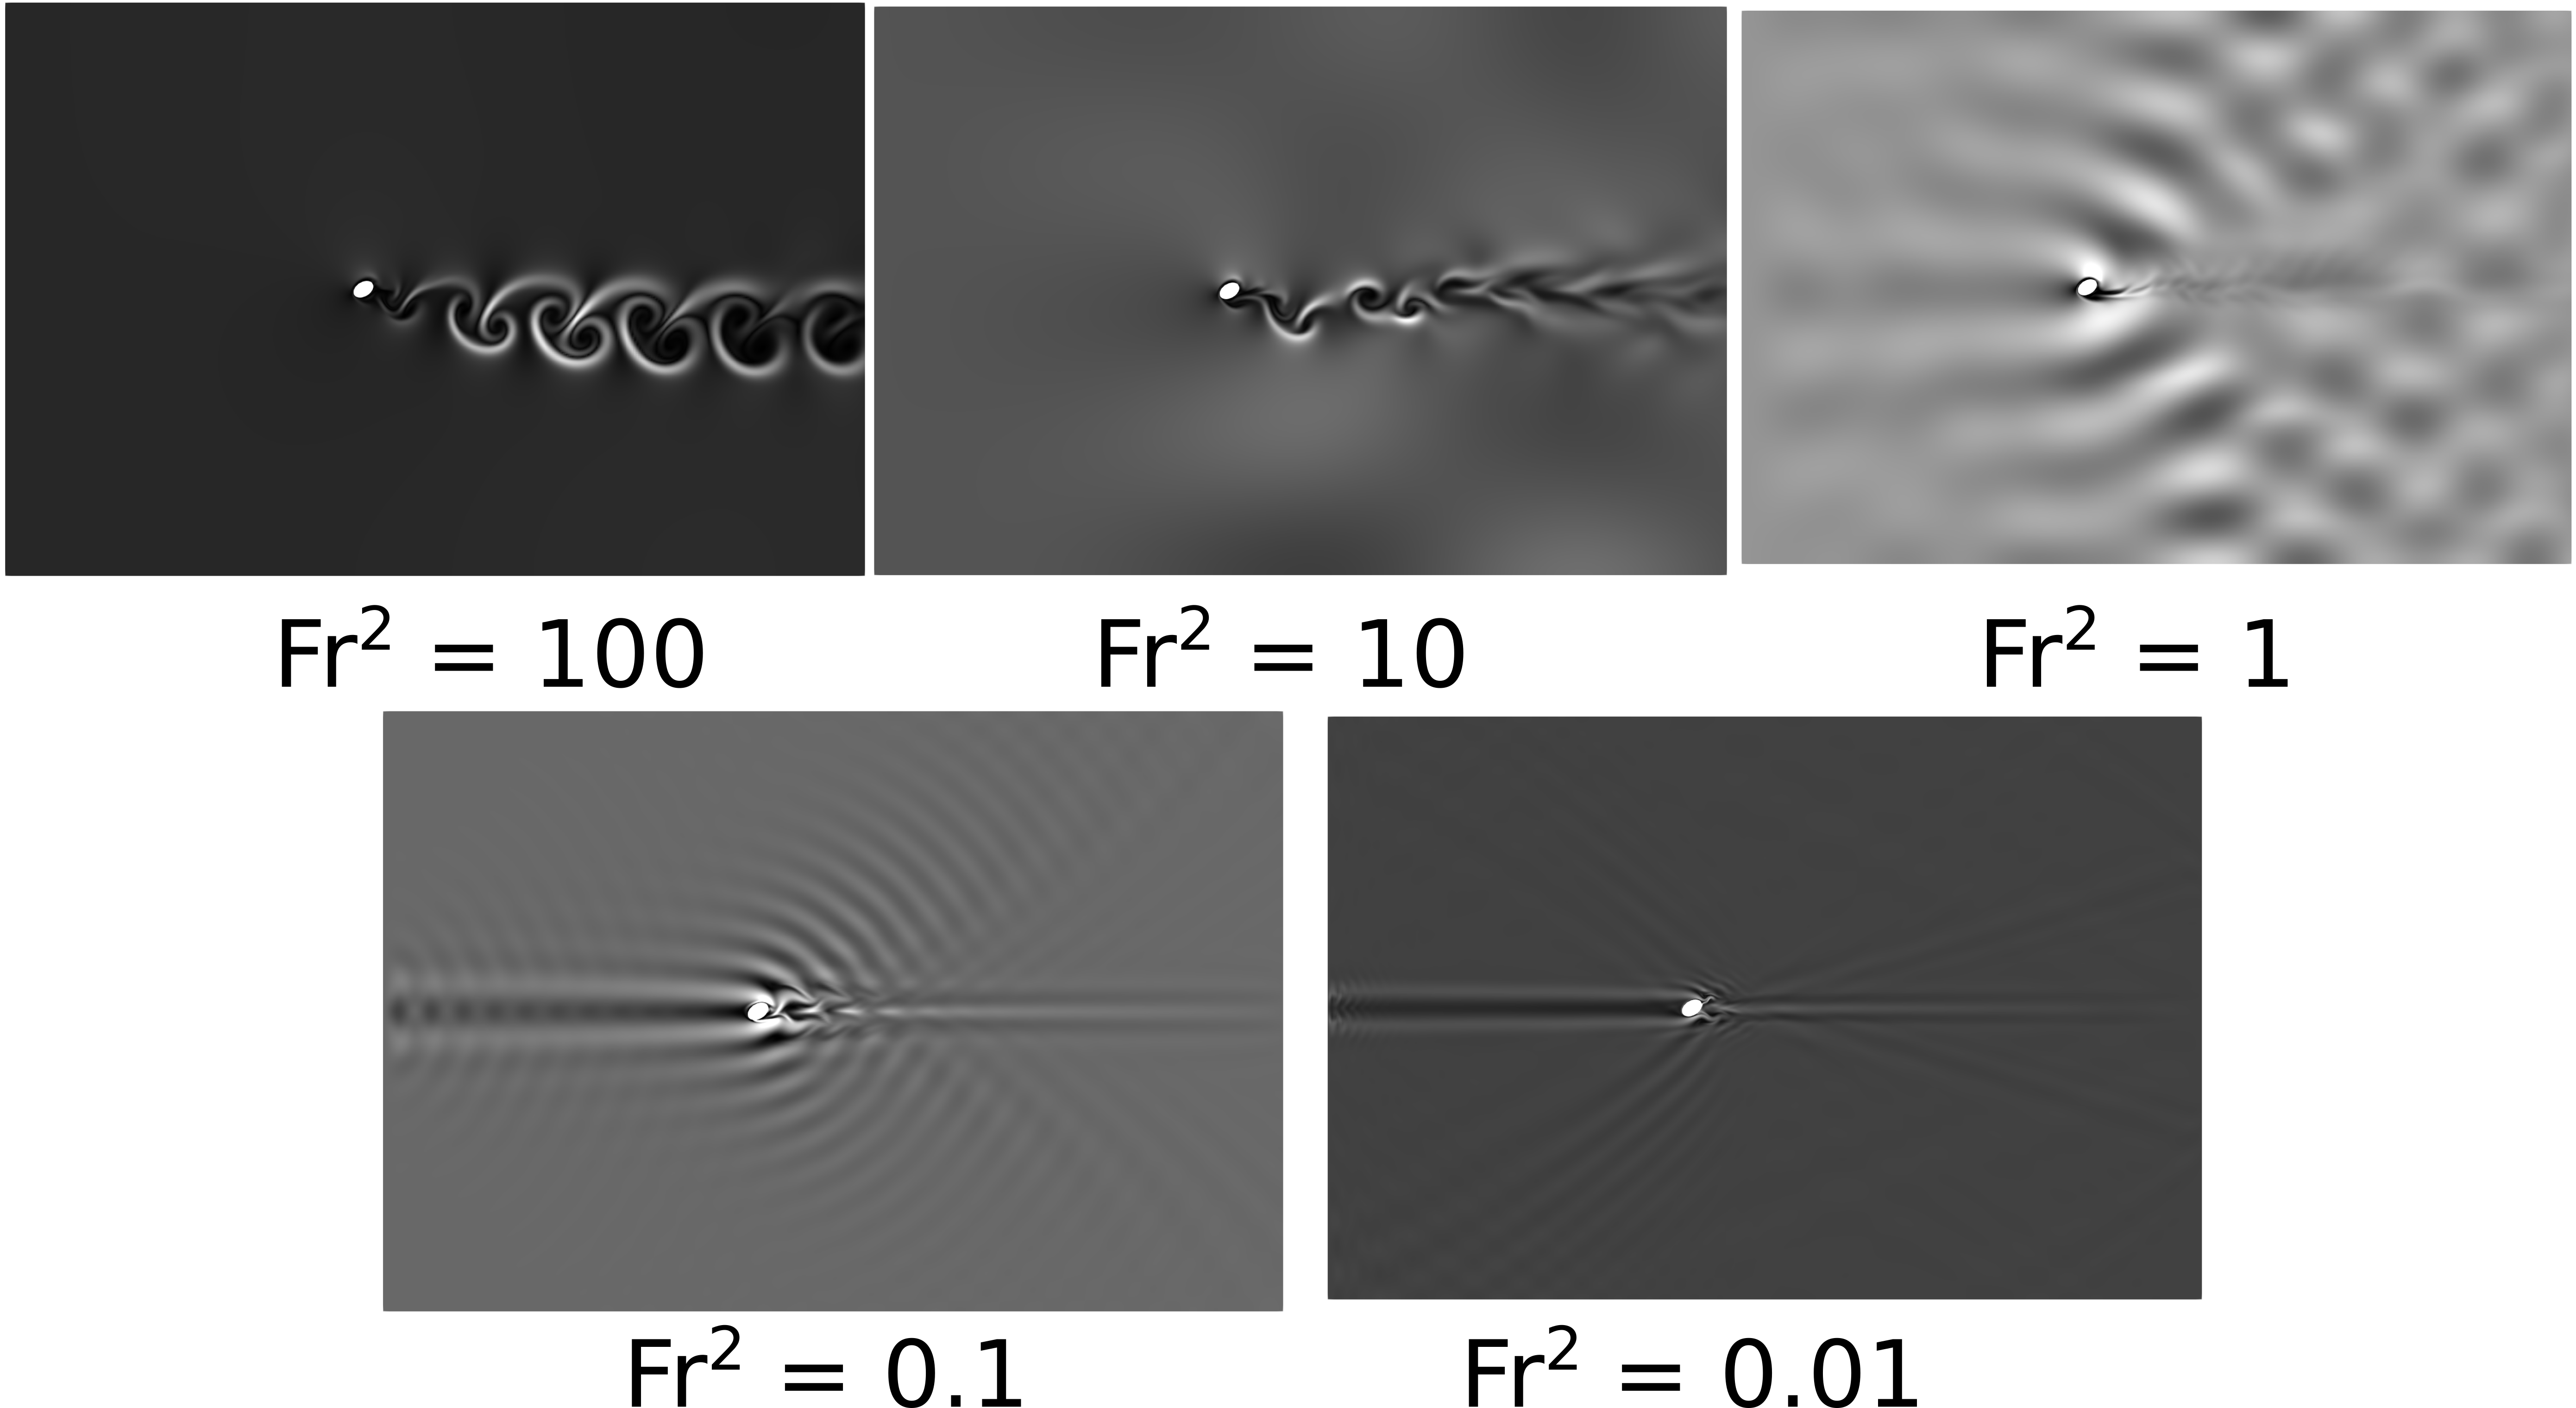
\includegraphics[width = \textwidth]{images/spinning_ellipse/schlerienar1p5.png}
    \caption{A comparison of the Schlerien fields for spinning ellipse where $AR = 1.5$}
    \label{fig:schlerienar1p5}
\end{figure}

\begin{figure}
    \centering
    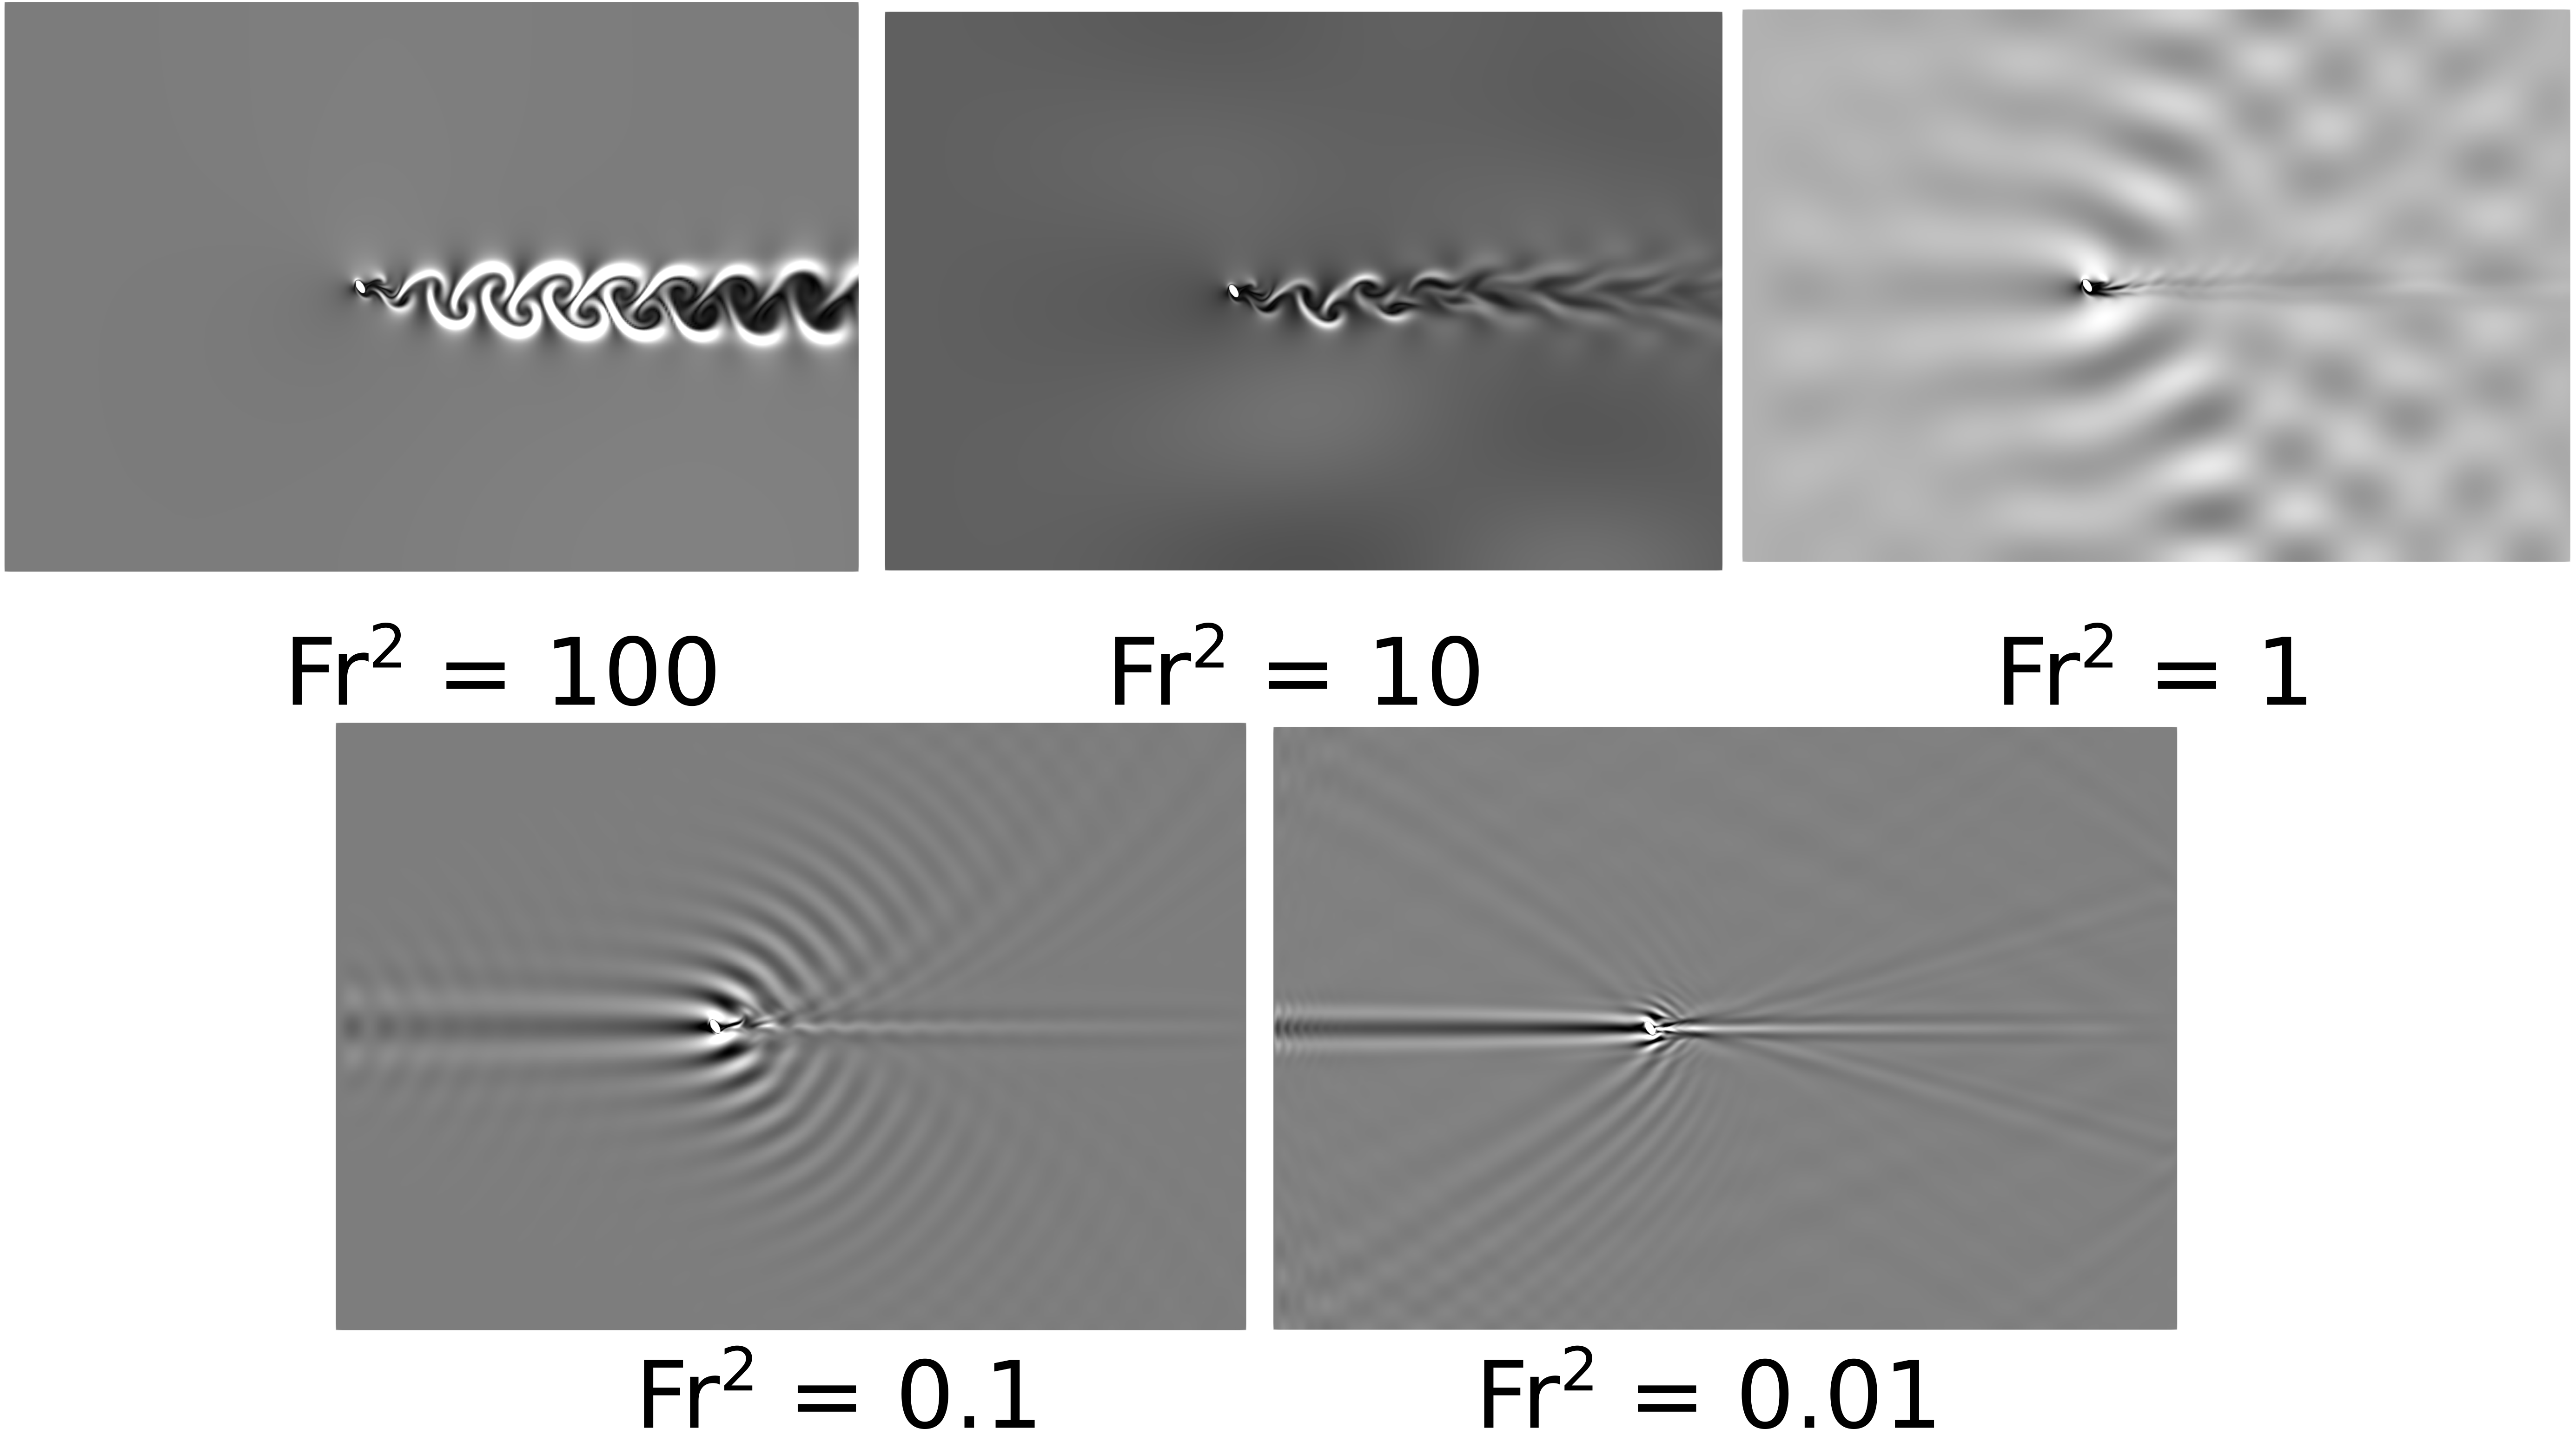
\includegraphics[width=\textwidth]{images/spinning_ellipse/schlerienar0p5.png}
    \caption{A comparison of the Schlerien fields for spinning ellipse where $AR = 0.5$}
    \label{fig:schlerienar0p5}
\end{figure}
